\section{Diagnostic de l'état de santé des batteries}
Pour commencer avec les batteries, un indicateur d'état de santé doit tout d'abord être choisi en accord avec les états de santé présents dans la littérature ainsi qu'avec le cas d'application du micro-réseau. La méthode de diagnostic permettant d'extraire cette valeur d'état de santé sera ensuite choisie puis appliquée. Les résultats du diagnostic de l'état de santé des batteries seront finalement présentés.
\subsection{Choix de l'indicateur d'état de santé}
Les indicateurs d'état de santé les plus répandus pour les batteries sont la capacité, en comparaison avec la capacité initiale, ainsi que la résistance interne, en comparaison avec la résistance interne initiale. La résistance interne est un paramètre directement corrélé avec la puissance que peut fournir la batterie \cite{noura_review_2020}. Dans le cadre du micro-réseau électrique, la batterie est utile pour ses capacités à stocker de l'énergie à court-terme. Ses caractéristiques de puissance passent au second plan dans un cadre où les panneaux photovoltaïques fournissent la majeure partie de la puissance électrique lors des périodes de fortes demandes. La capacité est donc choisie comme indicateur de l'état de santé de la batterie, et le SoH est défini par : 
\begin{equation}
    \mathrm{SoH} = \frac{C}{C_0}
    \label{soh_bat}
\end{equation}
où $C$ est la capacité de la batterie, et $C_0$ est sa capacité initiale, lorsque celle-ci était neuve.


\subsection{État de l'art des méthodes d'estimation en ligne}
Une fois l'indicateur d'état de santé défini, il convient maintenant de s'intéresser aux méthodes permettant de le déterminer \cite{peng_review_2022}. 

\subsubsection{Détermination directe par \textit{current throughput}}\hfill \\
L'estimation de la capacité par mesure directe (\textit{Current Throughput} ou \textit{Coulomb Couting}) est la méthode la plus commune et simple pour déterminer l'état de santé. Elle consiste en général en la décharge à courant constant de la batterie de son état de charge complet vers son état de charge vide, défini par exemple par un seuil de tension (fig. \ref{coulomb_counting}).

\begin{figure}[h]
\centering
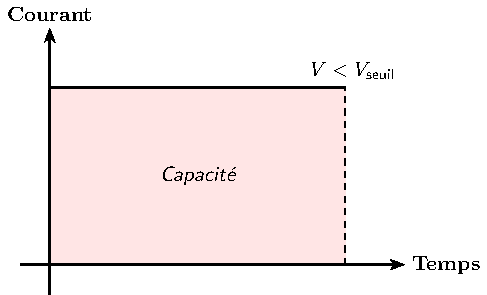
\includegraphics[width=.5\linewidth]{Chapitre 1/Diag_bat/Figures/coulomb_counting.pdf}
\caption{Mesure directe de capacité}
\label{coulomb_counting}
\end{figure}
\FloatBarrier

Les conventions pour la détermination de la capacité peuvent varier. Par exemple, l'\textit{International Electrotechnical Comission (IEC)} et l'\textit{International Organisation for Standardization (ISO)} prévoient des courants de décharge de 1C pour les applications de haute puissance (comme les véhicules hybrides), contre $\frac{C}{3}$ pour les batteries de haute énergie (véhicules complètement électriques) \cite{noauthor_iec_nodate}\cite{noauthor_iso_nodate}. Un courant plus faible offre une mesure plus précise en réduisant la chute de tension, mais s'obtient au détriment de la vitesse de diagnostic. Les conditions environnementales sont également strictes : l'IEC préconise 12h de repos avant test pour garantir la stabilisation thermique \cite{noauthor_iec_nodate}. Ces contraintes fortes, couplées au fait qu'une décharge complète est intrinsèquement dégradante pour la cellule, limitent l'utilisation de cette méthode en ligne. Elle reste cependant, par construction, l'approche de référence.

\subsubsection{Détermination de paramètres équivalents}\hfill \\
\paragraph{Méthodes basées sur les pulsations de courant} \hfill \\
Les méthodes basées sur les pulsations de courant permettent d'accéder simplement à un paramètre clé de la batterie. Elles consistent à appliquer une ou plusieurs pulsations de courant et à observer la réponse en tension pour en déduire l'état de la cellule (fig. \ref{current_pulse}).  

\begin{figure}[h]
\centering
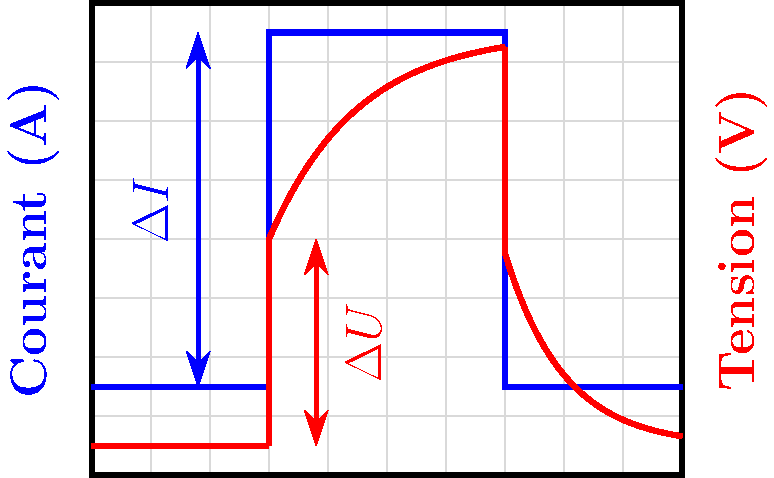
\includegraphics[width=.5\linewidth]{Chapitre 1/Diag_bat/Figures/current_pulse.pdf}
\caption{Pulsation de courant dans une batterie}
\label{current_pulse}
\end{figure}
\FloatBarrier

La résistance interne est ainsi rapidement accessible. Étant directement liée à la puissance délivrable et fortement corrélée à la capacité, elle constitue un bon indicateur. Néanmoins, cette mesure est très dépendante du courant de test, de la température et de l'état de charge \cite{stroe_degradation_2018}\cite{wen_online_2020}\cite{du_information_2022}. Cette méthode n'en demeure pas moins populaire pour sa rapidité d'exécution et sa facilité de mise en \oe uvre \cite{meng_lithium-ion_2018}.

\paragraph{Spectroscopie d'impédance électrochimique} \hfill \\
La spectroscopie d'impédance électrochimique (SIE) est une technique reconnue pour caractériser finement le vieillissement \cite{zhang_identifying_2020}\cite{jiang_comparative_2022}. Elle consiste à appliquer un signal sinusoïdal de fréquence variable afin d'en déduire une impédance complexe équivalente (fig. \ref{eis}).

\begin{figure}[h]
\centering
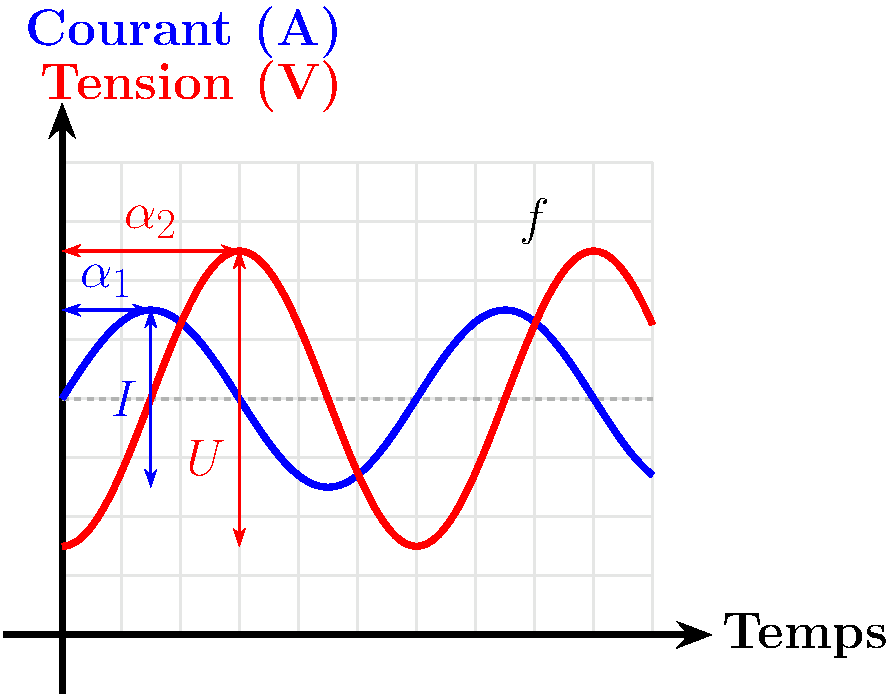
\includegraphics[width=.5\linewidth]{Chapitre 1/Diag_bat/Figures/eis.pdf}
\caption{Évolutions sinusoïdales du courant et de la tension dans une batterie au cours d'une SIE}
\label{eis}
\end{figure}
\FloatBarrier

Le balayage en fréquences permet d'obtenir un diagramme de Nyquist (mettant en relation partie réelle et partie imaginaire inversée) dont la forme évolue nettement avec le vieillissement (fig. \ref{nyquist_aging}). 

\begin{figure}[h]
\centering
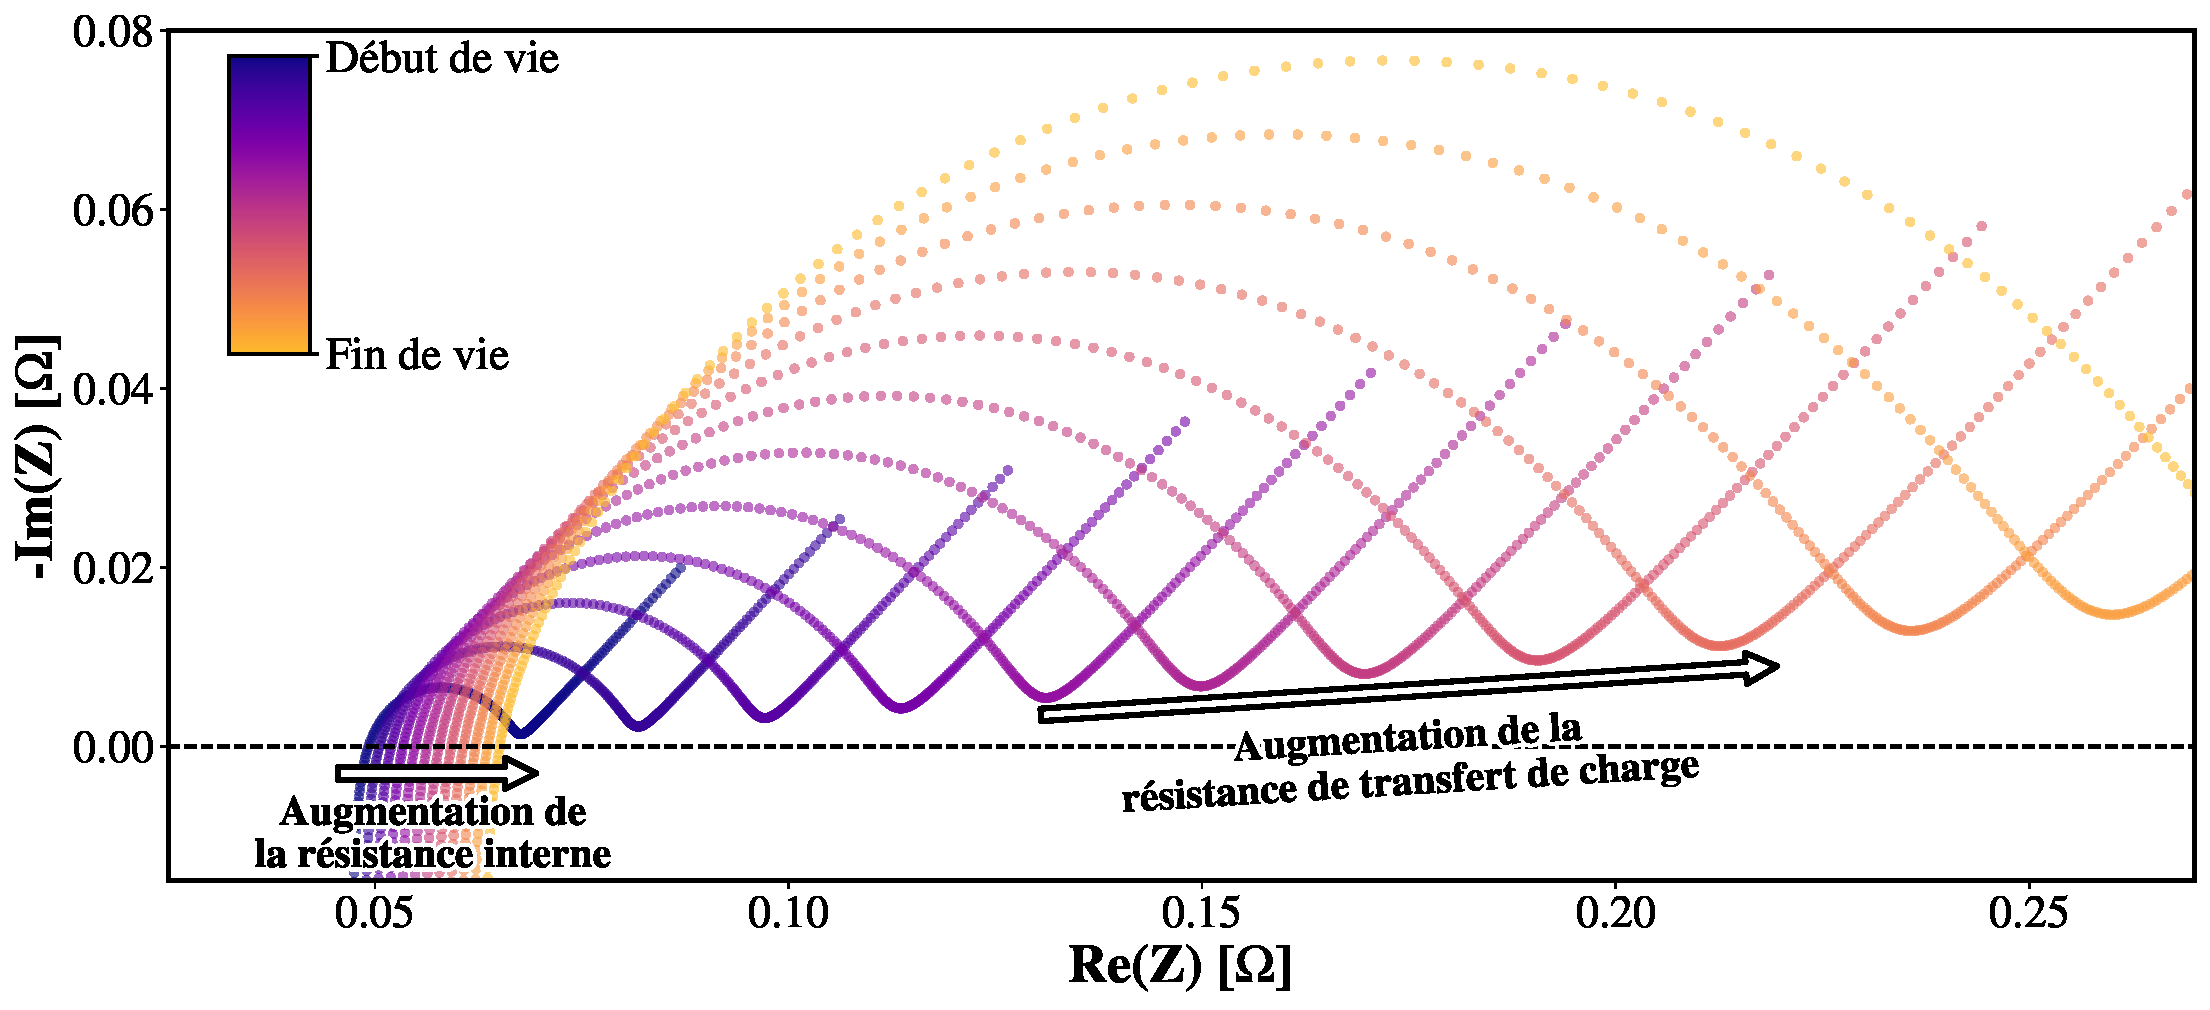
\includegraphics[width=.8\linewidth]{Chapitre 1/Diag_bat/Figures/nyquist_aging.pdf}
\caption{Évolution d'un diagramme de Nyquist avec le vieillissement}
\label{nyquist_aging}
\end{figure}
\FloatBarrier

Cette évolution peut être directement traduite sous la forme de circuits électriques équivalents (\textit{Equivalent Circuit Model}, ou ECM, fig. \ref{ecm_bat}), incluant des inductances, résistances et éléments à phase constante (\textit{CPE}) \cite{zhang_electrochemical_2022}. 

\begin{figure}[h]
\centering
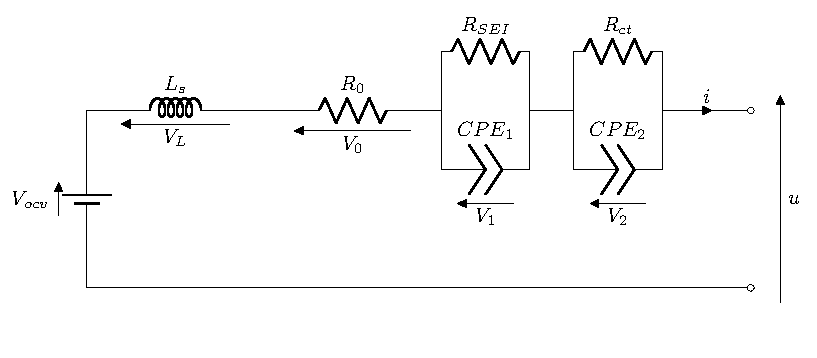
\includegraphics[width=.8\linewidth]{Chapitre 1/Diag_bat/Figures/ecm_bat.pdf}
\caption{Circuit électrique équivalent de batterie}
\label{ecm_bat}
\end{figure}
\FloatBarrier

Chaque zone du diagramme de Nyquist correspond alors à un paramètre spécifique du modèle (fig. \ref{nyquist}), ce qui permet d'isoler et de quantifier physiquement la source de la dégradation. 

\begin{figure}[h]
\centering
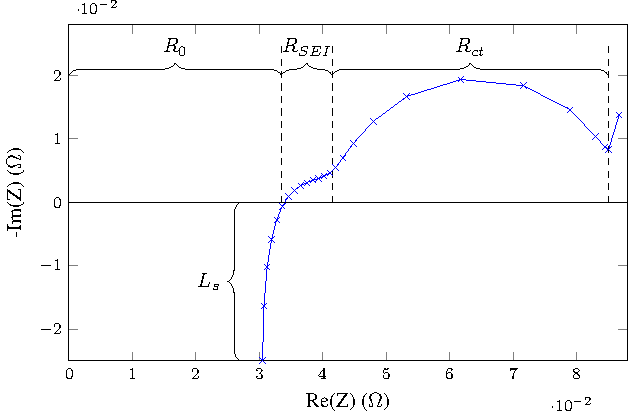
\includegraphics[width=.8\linewidth]{Chapitre 1/Diag_bat/Figures/nyquist.pdf}
\caption{Diagramme de Nyquist et relation avec les paramètres du circuit}
\label{nyquist}
\end{figure}
\FloatBarrier
La SIE offre un diagnostic riche, mais sa mise en \oe uvre peut être difficile en ligne et requiert l'utilisation d'un spectromètre, matériel potentiellement onéreux et encombrant.

\subsubsection{Autres méthodes}\hfill 
\paragraph{Courbes incrémentales et différentielles}\hfill \\
L'analyse des courbes dérivées est une méthode indirecte très répandue. La courbe incrémentale en capacité ($IC = \frac{\mathrm{d}Q}{\mathrm{d}V}$) est particulièrement pertinente car sa forme évolue avec le vieillissement de la batterie \cite{lin_multi-feature-based_2022}\cite{xiaopeng_battery_2020}. Contrairement à la mesure directe, il n'est pas nécessaire de couvrir toute la plage d'états de charge pour observer les décalages des pics caractéristiques (fig. \ref{ic_curve}) \cite{han_comparative_2014}. 

\begin{figure}[h]
\centering
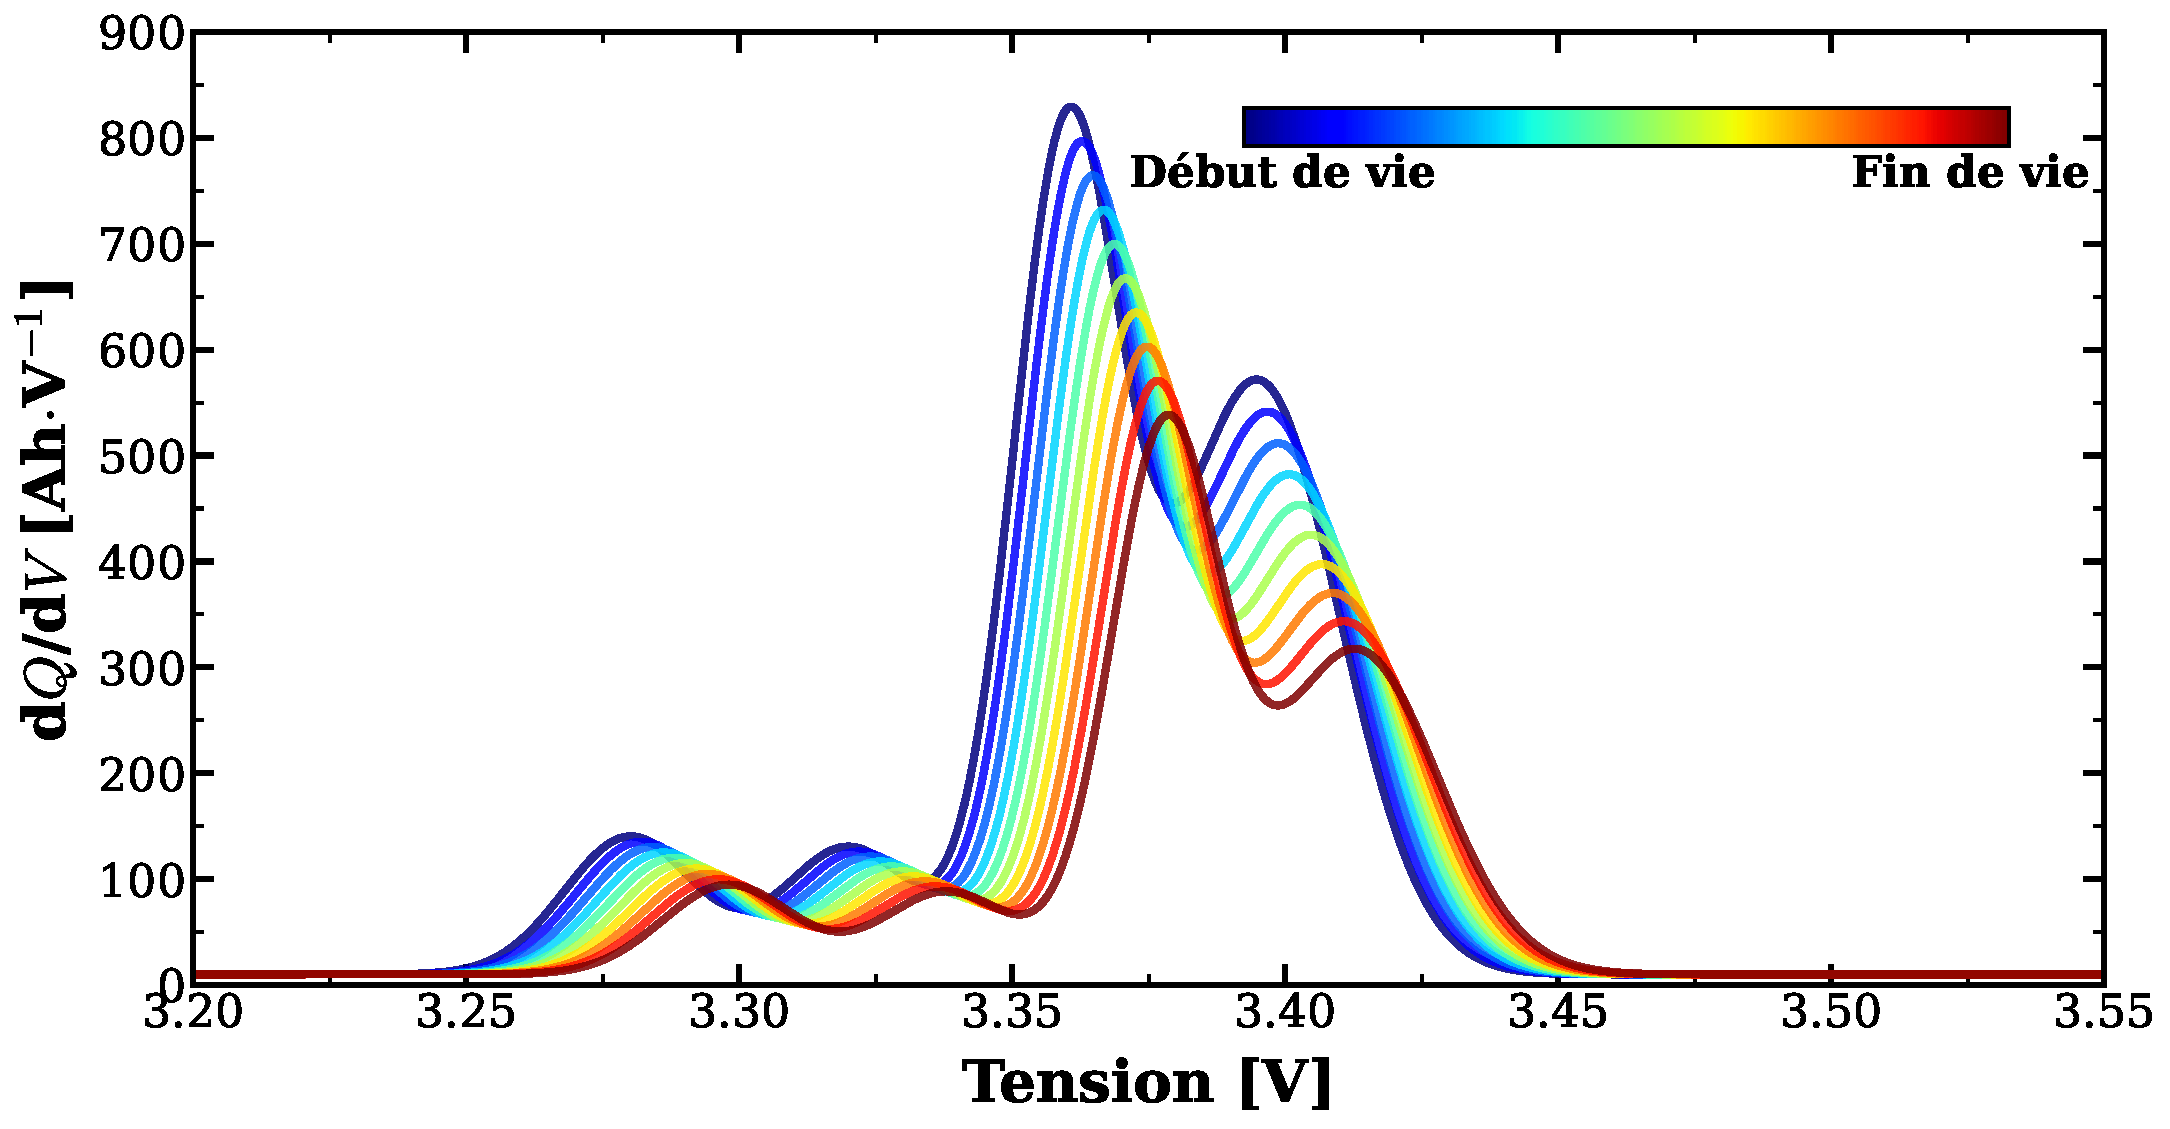
\includegraphics[width=\linewidth]{Chapitre 1/Diag_bat/Figures/ic_curve.pdf}
\caption{Évolution d'une courbe incrémentale en capacité}
\label{ic_curve}
\end{figure}
\FloatBarrier

Ce décalage est notamment relié à la perte de matériau actif et à la perte de lithium utilisable \cite{jiang_state_2018}. De manière analogue, la courbe différentielle en tension ($DV = \frac{\mathrm{d}V}{\mathrm{d}Q}$) \cite{en7084895}\cite{honkura_capacity-fading_2011} et la courbe différentielle en température ($DT = \frac{\mathrm{d}T}{\mathrm{d}V}$) \cite{wu_differential_2015} exploitent ces mêmes principes. La méthode basée sur la température s'avère particulièrement complémentaire lors de forts courants de charge ou décharge, car elle met en exergue l'évolution des pertes ohmiques liées à l'âge de la cellule \cite{zhang_research_2022}\cite{yang_lithium-ion_2022}.


\paragraph{Méthodes basées sur l'état de charge et observateurs} \hfill \\
Le diagnostic par estimation indirecte repose sur l'équation fondamentale du \textit{Coulomb counting} (eq. \ref{eq_coulomb_couting}) :
\begin{equation}
    \text{SoC}(t_1) = \text{SoC}(t_0) + \frac{1}{3600C_{bat}}\int_{t_0}^{t_1} i(t) \mathrm{d}t
    \label{eq_coulomb_couting}
\end{equation}
La tension en circuit ouvert (\textit{open-circuit voltage}, ou OCV) n'étant pas directement mesurable en usage réel, il est nécessaire d'utiliser un modèle de batterie, typiquement de type $nRC$ avec $n \in \{1, 2\}$ (fig. \ref{nrc}) \cite{lai_comparative_2018}. 

\begin{figure}[h]
\centering
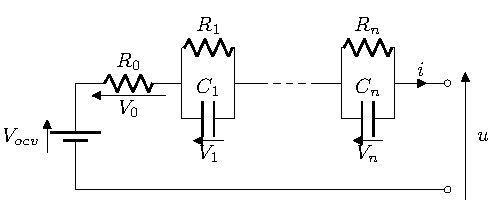
\includegraphics[width=.8\linewidth]{Chapitre 1/Diag_bat/Figures/nrc.pdf}
\caption{Circuit équivalent de batterie type $nRC$}
\label{nrc}
\end{figure}
\FloatBarrier

Dans ces modèles équivalents, la capacité a une influence directe sur le comportement dynamique. Il est alors possible d'estimer cette capacité conjointement avec le SoC via des méthodes de filtrage comparant les mesures réelles aux prédictions du modèle. On retrouve des algorithmes tels que les moindres carrés récursifs \cite{wei_state_2020}, le filtre de Kalman étendu (\textit{Extended Kalman Filter}, ou EKF) \cite{shen_co-estimation_2018}\cite{qian_hybrid_2021}, le filtre de Kalman à point sigma (\textit{Sigma Point Kalman Filter}, SPKF) pour mieux gérer les non-linéarités \cite{liu_online_2022}, ou encore le filtrage particulaire (\textit{Particle Filter}, PF) stochastique \cite{cai_data-driven_2022}. Bien que performantes, ces approches voient leur précision directement liée à la fidélité du modèle choisi.

\paragraph{Méthodes basées sur les données} \hfill \\
Formant une philosophie distincte, les méthodes basées sur les données considèrent le système comme une "boîte noire". Le diagnostic ne repose plus sur une connaissance physique explicite mais sur l'analyse algorithmique de grandes quantités de données pour lier le vieillissement aux caractéristiques mesurées \cite{peng_review_2022}. 

\subparagraph{Réseaux de neurones et Apprentissage profond} \hfill \\
Les réseaux de neurones utilisent des couches successives de neurones artificiels pour interpoler les données d'entrée (mesures) vers une sortie (diagnostic) après une phase d'entraînement \cite{zhao_lithium-ion_2022}\cite{zhou_battery_2015}. L'apprentissage profond (\textit{Deep Learning}) en est une extension plus complexe. Utilisant des structures avancées comme les réseaux convolutifs \cite{gu_novel_2023} ou récurrents \cite{ma_novel_2022}, ils offrent une très grande précision mais requièrent des jeux de données d'apprentissage massifs.

\subparagraph{Machines à vecteur de support et méthodes bayésiennes} \hfill \\
Les machines à vecteur de support (\textit{Support Vector Machine}, ou SVM) sont des algorithmes séparant les données via un hyperplan optimal afin d'effectuer de la classification ou de la régression robuste \cite{xie_aviation_2014}\cite{wang_co-estimation_2021}. Les approches bayésiennes (comme les processus gaussiens), quant à elles, actualisent de manière probabiliste les hypothèses de diagnostic à mesure que de nouvelles données sont observées \cite{liu_data-driven_2021}\cite{chen_lithium-ion_2021}.

\subsubsection{Conclusion}
Un résumé des différentes approches est disponible dans le tableau \ref{table_diag_bat} :

\begin{table}[h]
\centering
\caption{Synthèse des méthodes de diagnostic de l'état de santé \vspace{0.2cm}}
\begin{tabular}{M{3cm} M{4.8cm} M{3cm} M{3.5cm} }
\hline
\textbf{Catégories} & \textbf{Méthodes \& Références} & \textbf{Avantages} & \textbf{Inconvénients} \\
\hline \hline
Détermination directe 
& \textit{Coulomb counting} (Décharge complète) \cite{noauthor_iec_nodate}\cite{noauthor_iso_nodate} & Méthode de référence, précision élevée & Très chronophage, potentiellement dégradant \\
\hline
\multirow{3.5}{3cm}{\centering Extraction de paramètres équivalents } 
& Pulsations de courant \cite{stroe_degradation_2018}-\cite{meng_lithium-ion_2018} & Rapidité, très simple à implémenter & Sensible au SoC et à la température \\
\cline{2-4}
& Spectroscopie d'impédance électrochimique (SIE) \cite{zhang_identifying_2020}-\cite{zhang_electrochemical_2022} & Diagnostic très riche, peu intrusif & Spectromètre coûteux, complexe en ligne \\
\hline
\multirow{3.5}{3cm}{\centering Courbes différentielles et observateurs} 
& Courbes IC, DV et DT \cite{lin_multi-feature-based_2022}-\cite{yang_lithium-ion_2022} & Identification des modes de dégradation (LLI, LAM) & Très sensible au bruit de mesure \\
\cline{2-4}
& Modèles $nRC$ et Observateurs (EKF, SPKF, PF) \cite{shen_co-estimation_2018}-\cite{cai_data-driven_2022} & Estimation en temps réel, robuste au bruit & Très dépendant de la fidélité du modèle choisi \\
\hline
\multirow{4}{3cm}{\centering Méthodes basées sur les données } 
& Réseaux de neurones et \textit{Deep Learning} \cite{zhao_lithium-ion_2022}-\cite{gu_novel_2023} & \multirow{4.5}{2.5cm}{\centering Haute précision, s'affranchit de la physique du système} & \multirow{4.5}{2.5cm}{\centering Nécessite un volume massif de données, effet "boîte noire"} \\
\cline{2-2}
& Machines à vecteurs de support (SVM) \cite{xie_aviation_2014} &  &  \\
\cline{2-2}
& Méthodes bayésiennes (GP, RVM) \cite{liu_data-driven_2021}-\cite{chen_lithium-ion_2021} &  &  \\
\hline
\end{tabular}
\label{table_diag_bat}
\end{table}
\FloatBarrier

Au vu des différents avantages et inconvénients de toutes ces méthodes de diagnostic, il a été choisi d'utiliser une combinaison des méthodes basées sur les pulsations de courant et sur la spectroscopie d'impédance électrochimique. Ces deux méthodes ont les avantages d'être rapides à mettre en \oe uvre et sont donc adaptées à un contexte de diagnostic dans un micro-réseau qu'on souhaite le moins intrusif possible. Choisir deux méthodes complémentaires pour les mêmes batteries permet ici d'avoir un choix éclairé pour une approche qui peut être dépendante de la chimie des batteries ou de l'environnement des expériences. Cela permet également d'observer le comportement à la fois fréquentiel et impulsionnel des batteries, offrant ainsi une vue plus globale de leur dynamique. Pour l'application de ces méthodes, il est donc justifié de produire des données expérimentales sur des cellules de batteries afin d'observer le vieillissement et de quantifier la pertinence des approches choisies.

\subsection{Description de la campagne d'essais réalisée}
Dans le cadre de l'étude du vieillissement des batteries, des essais unicellulaires ont été effectués au laboratoire FEMTO-ST. Ces essais avaient pour objectif d'observer le vieillissement de cellules de batteries SAMSUNG ICR18650 (chimie Nickel-Manganèse-Cobalt, ou NMC) de capacité initiale 2.6Ah. Ces cellules étaient au nombre de cinq, trois d'entre elles étant testées seules et les deux autres étant assemblées en parallèle pour former un module. Ces essais ont pris la forme d'essais de vieillissement accélérés (\textit{Accelerated Stress Tests , ou AST}), composés de cycles de charge/décharge effectués en boucle pour approche un vieillissement réel de cellules de batterie. Ces périodes de vieillissement étaient ensuite suivies de caractérisations régulières, environ tous les 35 cycles. Ces caractérisations étaient à la fois statiques (mesure de capacité et pulsations de courant sous le forme de \textit{Hybrid Power Pulse Characterization}, ou HPPC), et dynamiques (spectroscopie d'impédance électrochimique). Un diagramme de flux représentant le déroulé de ces essais est présent en figure \ref{essais}.
\begin{figure}[h]
\centering
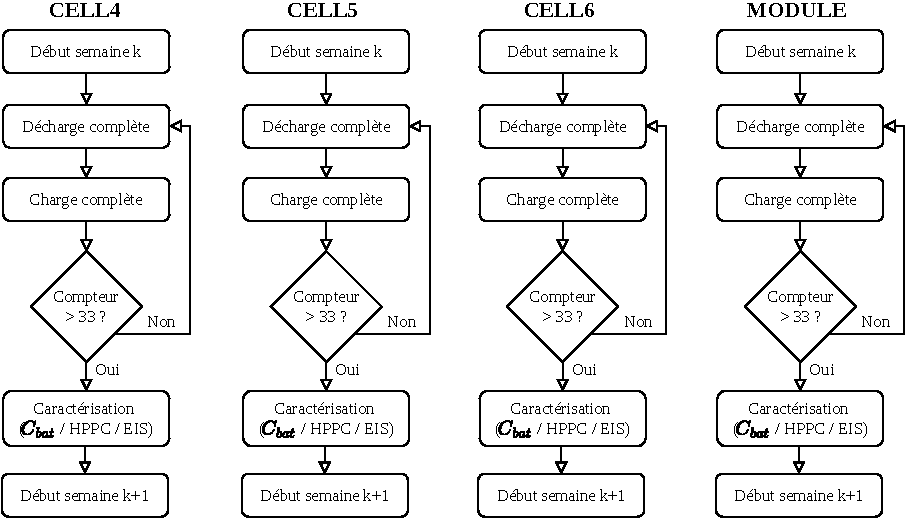
\includegraphics[width=\linewidth]{Chapitre 1/Diag_bat/Figures/flowchart_essais2.pdf}
\caption{Diagramme de flux des essais sur batteries}
\label{essais}
\end{figure}
\FloatBarrier
Cette caractérisation régulière permet de suivre l'évolution des caractéristiques des cellules de batterie au cours de leur cycle de vie. Dans un objectif de représenter une première et seconde vie des batteries, une première série de cycles a été effectuée jusqu'à une dégradation d'environ 30\% de la capacité initiale, qui a été suivie d'une pause complète de quelques semaines puis une deuxième série de tests jusqu'à une dégradation de 80\% de la capacité initiale. 

\subsubsection{Équipements}
Ces essais ont eu lieu sur un banc de décharge de batteries unicellulaires de la marque CHROMA\textsuperscript{\textregistered}, permettant d'appliquer des programmes d'instructions électriques à des batteries pour mener ces essais à bien. Le banc d'essai utilisé est présenté en figure \ref{chroma}.
\begin{figure}[h]
\centering
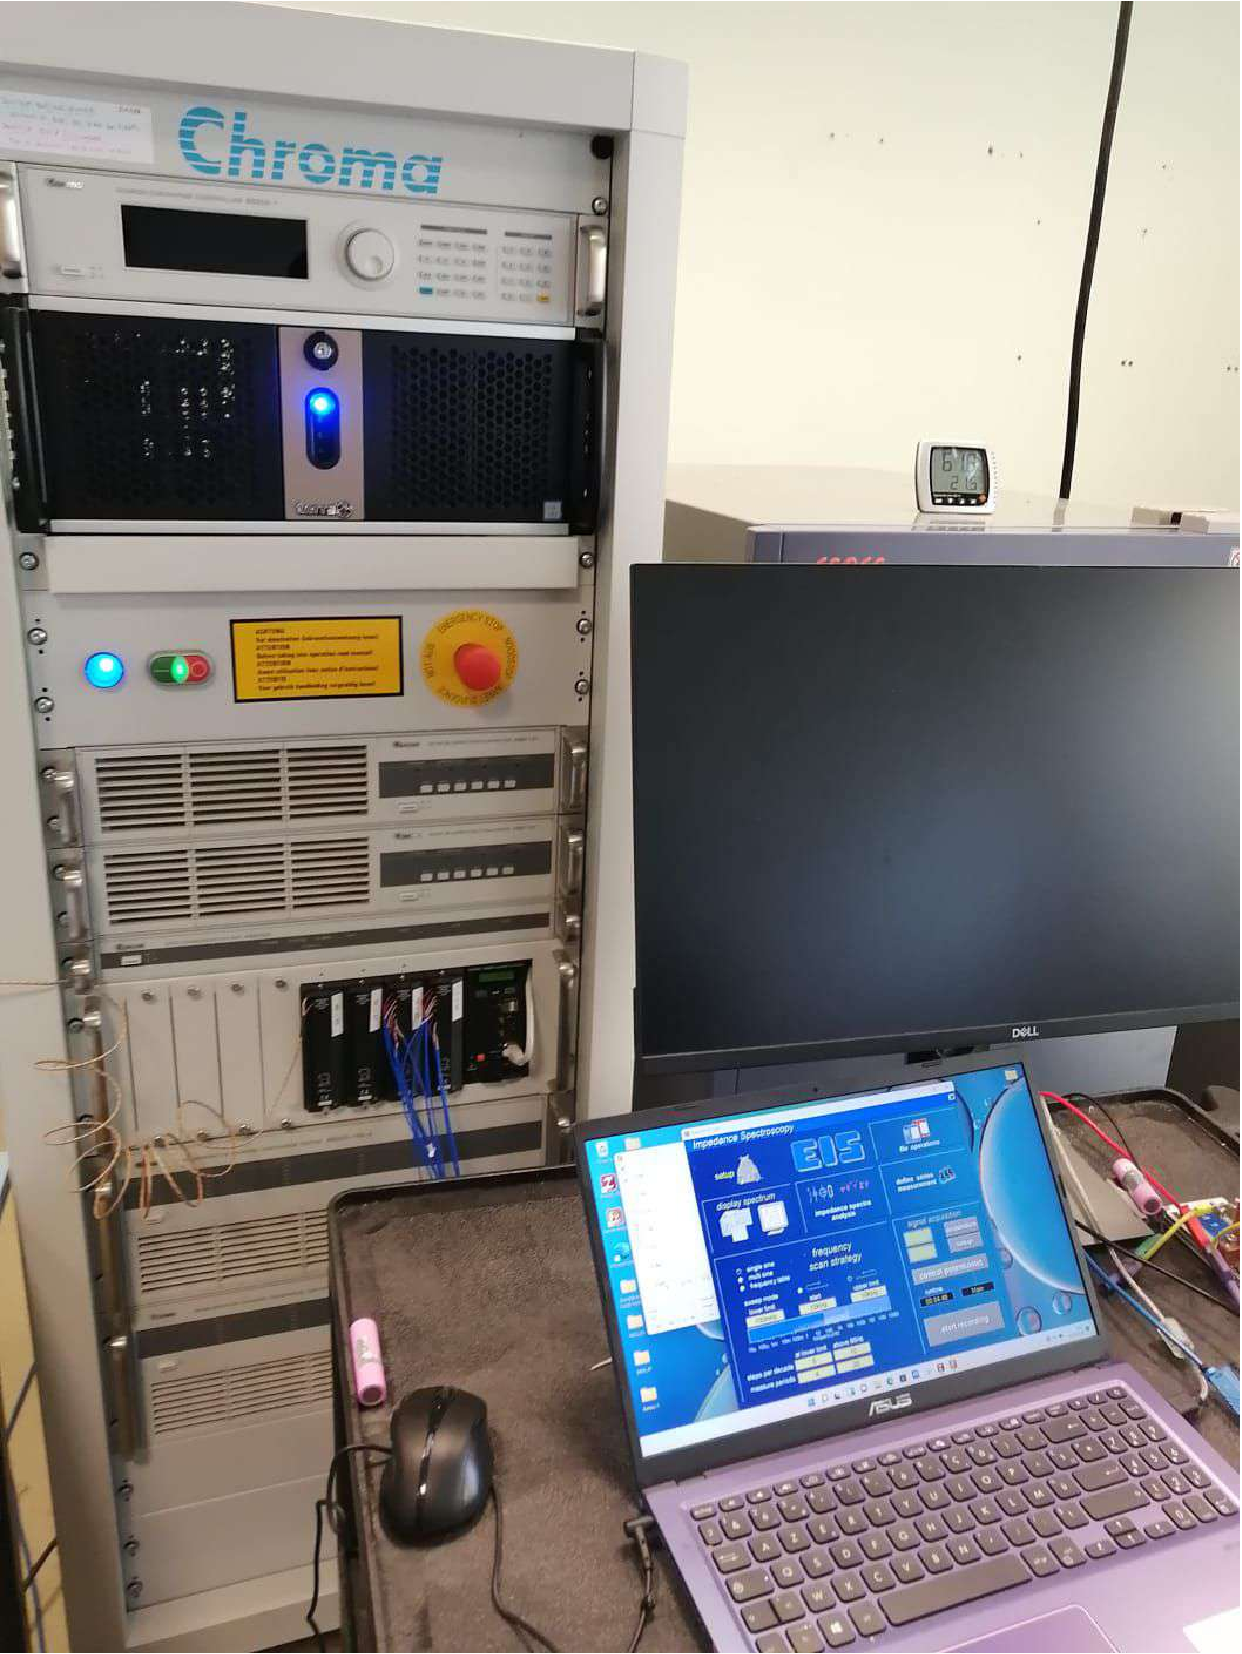
\includegraphics[width=.8\linewidth]{Chapitre 1/Diag_bat/Figures/chroma.pdf}
\caption{Banc d'essai CHROMA 17020}
\label{chroma}
\end{figure}
\FloatBarrier
Ce banc d'essai a été utilisé pour les tests de vieillissement accélérés, ainsi que pour les caractérisations par pulsations de courant. Les caractérisations dynamiques par spectroscopie d'impédance électrochimique ont été réalisées grâce à un spectromètre commercial de la marque Zahner\textsuperscript{\textregistered} \ (fig. \ref{spectrometer}).
\begin{figure}[h]
\centering
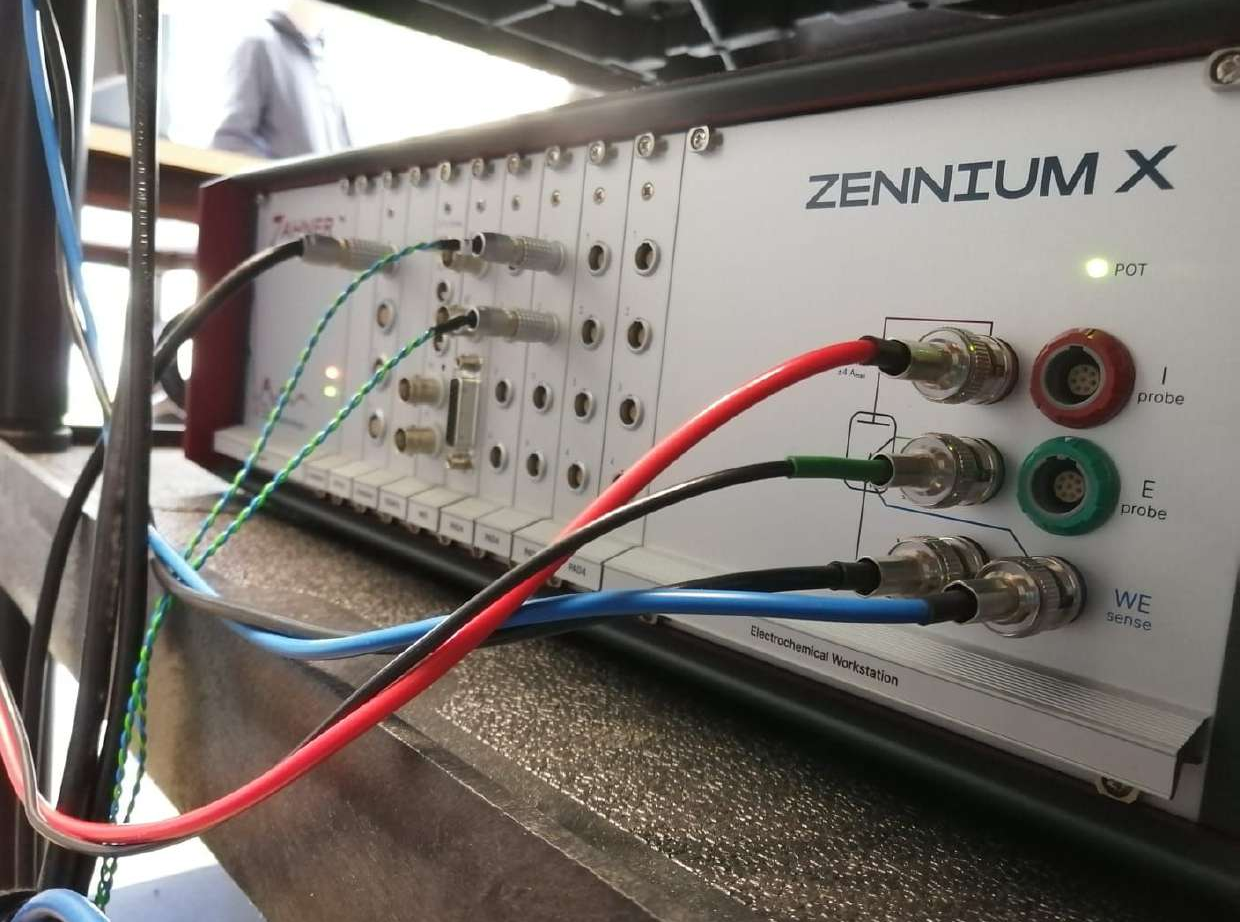
\includegraphics[width=.8\linewidth]{Chapitre 1/Diag_bat/Figures/spectrometer.pdf}
\caption{Banc d'essai Zahner Zennium X}
\label{spectrometer}
\end{figure}
\FloatBarrier

\subsubsection{Protocoles}
\paragraph{Tests de vieillissements accélérés}\hfill \\
Les tests de vieillissement accéléré (AST) prenaient ici la forme de 33 cycles de charge/décharge espacés de périodes de repos de quelques minutes. Avoir 33 cycles permettait de faire des caractérisations toutes les semaines, avec une dégradation de la capacité de l'ordre de quelques pourcents. Ainsi, cela était un compromis entre une fréquence trop élevée lourde en temps à consacrer aux caractérisations et une fréquence trop faible ne permettant pas de suivre aisément la dégradation des caractéristiques de la batterie. Les courant imposés étaient de 1C et étaient appliqués jusqu'à atteindre un seuil de tension (maximale ou minimale selon si c'était en charge ou décharge). Cette approche permettait ainsi d'avoir un vieillissement plus rapide qu'en conditions réelles. Une des limitations de cette approche reste cependant que les cellules de batterie ne sont soumises qu'à des courants constants, peu représentatifs de la réalité et des pics de courant qui peuvent les endommager.

\paragraph{Mesure de la capacité}\hfill \\
Une fois chaque période de vieillissement effectuée, la première quantification de la dégradation qui est mesurable est l'évolution de la capacité. Cette capacité est simplement mesurée à l'aide d'une décharge complète à 1C ainsi qu'une mesure du courant puis une intégration de celui-ci (méthode dite de \textit{coulomb counting}, fig. \ref{coulomb_counting}). C'est cette mesure qui permettait de voir la détérioration de la capacité au fil des semaines.

\paragraph{Spectroscopie d'impédance électrochimique}\hfill \\
Les spectroscopies d'impédance électrochimique étaient appliquées toutes les semaines, à la suite des mesures de capacité pour avoir un suivi suffisamment échantillonné de l'évolution des spectre de Nyquist. Les caractéristiques des batteries étant très dépendantes de l'état de charge actuel, ces spectroscopies ont été effectuées sur chaque cellule à quatre état de charge différents, à savoir 100\%, 75\%, 50\% et 25\%.

\paragraph{\textit{Hybrid Power Pulse Characterization}}\hfill \\
Les tests HPPC étaient égalemnt appliqués toutes les semaines, ce qui était la dernière pièce de la caractérisation complète des batteries. Des impulsions de courant à la fois positives et négatives, et d'amplitude de 1C et 0,5C ont été appliquées à toutes les cellules et pour les mêmes quatre états de charge distincts. Un exemple de profil HPPC est présenté en figure \ref{hppc}. 
\begin{figure}[h!]
    \centering
        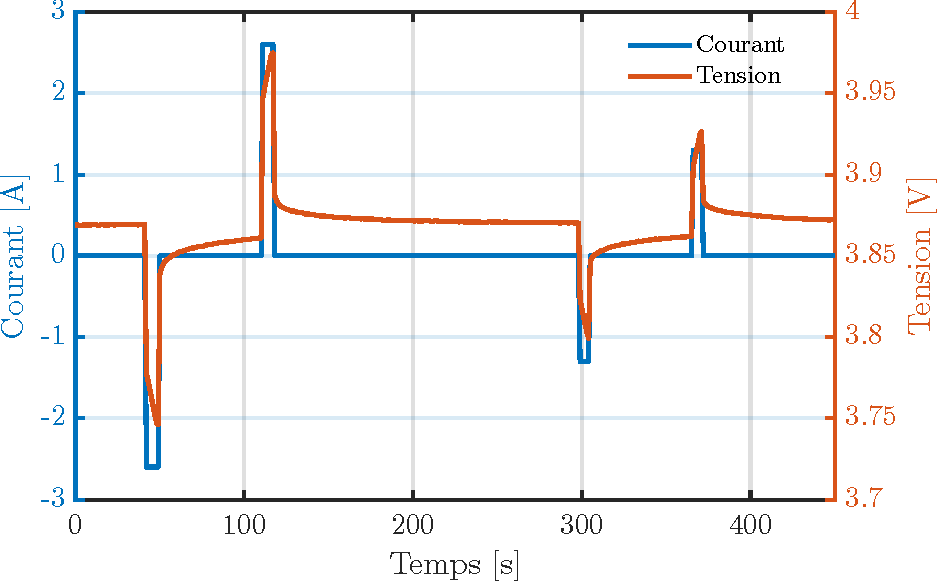
\includegraphics[width=.8\linewidth]{Chapitre 1/Diag_bat/Figures/VI_plot_CELL4_WEEK1_SOC75.pdf}
    \caption{Test HPPC appliqué à une cellule de batterie}
    \label{hppc}
\end{figure}
\FloatBarrier

\subsection{Traitement des données \& détermination de la capacité}
Les deux méthodes choisies pour la détermination de la capacité sont les pulsations de courant par HPPC ainsi que la spectroscopie d'impédance électrochimique. Dans cette partie, les résultats des essais expérimentaux seront présentés ainsi que le traitement des données pour en faire le diagnostic des batteries.

\subsubsection{Présentation des données}
Les essais en vieillissement des batteries se sont déroulés sur une trentaine de semaines et sur quatre éléments différents (trois cellules simples et un module de deux cellules). Les données récoltées prennent la forme de séries temporelles que ce soit pendant les périodes de vieillissement accélérés ou pendant les périodes de caractérisation.  Celles-ci sont organisées en trois catégories distinctes : les mesures de capacité "brutes", par décharge complète, les données des tests HPPC, les données des SIE. Ici, les mesures de capacité attestent du vieillissement des batteries (comme par exemple en figure \ref{capa_cell5}), et sont donc les valeurs qui chercheront à être estimées par les méthodes de diagnostic suivantes. Les valeurs de capacité se présentent simplement sous la forme de série temporelle.
\begin{figure}[h!]
    \begin{minipage}{.51\linewidth}
    \centering
    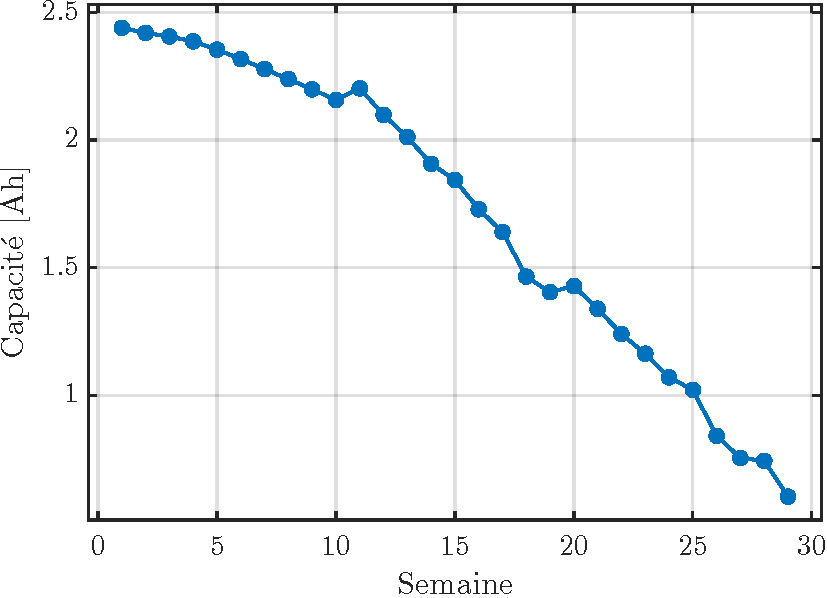
\includegraphics[width=\linewidth]{Chapitre 1/Diag_bat/Figures/Capacity_Plot.pdf}
    \end{minipage}%
    \hfill
    \begin{minipage}{.48\linewidth}
    \centering
    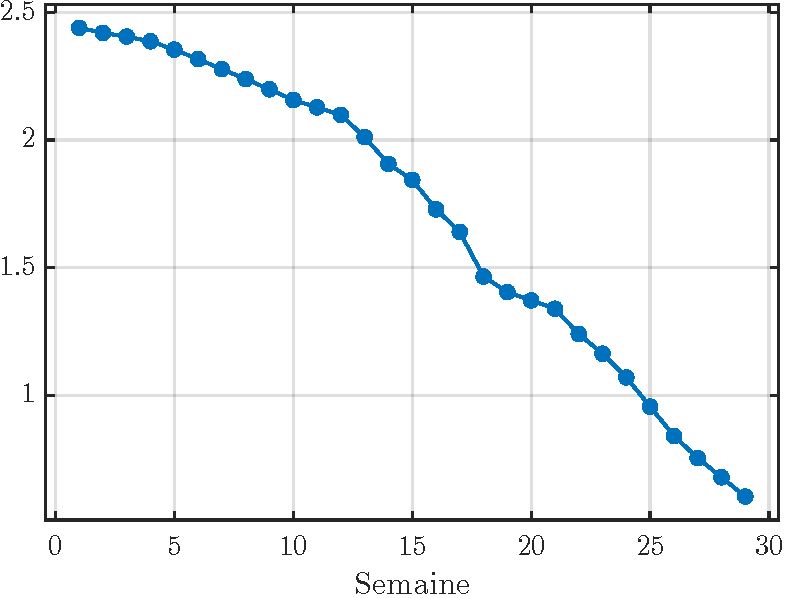
\includegraphics[width=\linewidth]{Chapitre 1/Diag_bat/Figures/Capacity_Plot_filtered.pdf}
    \end{minipage}
    \caption{Évolution de la capacité de la cellule 5 au cours des semaines d'essais (gauche) et filtrée (droite)}
    \label{capa_cell5}
\end{figure}
\FloatBarrier
Il est intéressant de noter également que dans ces mesures de capacité, il y a des mesures a priori aberrantes où la capacité ré-augmente localement. Ces données étant sans doute issues d'erreurs de mesures ponctuelles ou de changements mineurs d'environnement de travail, elles sont effacées à la main par lissage linéaire (fig. \ref{capa_cell5} droite). Les données suivantes représentent les deux méthodes de diagnostic qui chercheront à approcher les valeurs de capacité brutes. Pour chacune des deux méthodes les mesures ont été faites à quatre niveaux d'états de charge différents : 25\%, 50\% 75\% et 100\%. Les différents niveaux d'états de charge étaient atteints par décharge depuis l'état de charge complet et une intégrale de courant pour déterminer la capacité vidée. \\
Les données des spectroscopies d'impédance sont des données dans le domaine fréquentiel cette fois, et non pas temporel. Elles prennent donc la forme de trois vecteurs. Un premier vecteur de fréquence, allant de la dizaine de millihertz vers la dizaine de kilohertz. À chaque fréquence sont associées des données d'impédances réelles et imaginaire, calculées à partir des mesures en tension et courant. Ces données d'impédance permettent alors de reconstituer les classiques diagrammes de Bode ou de Nyquist (fig. \ref{nyquist}). Un exemple pour une cellule de tous les diagrammes de Nyquist au cours de sa vie est présenté en figure \ref{nyquist_aging2}. 
\begin{figure}[h!]
    \centering
        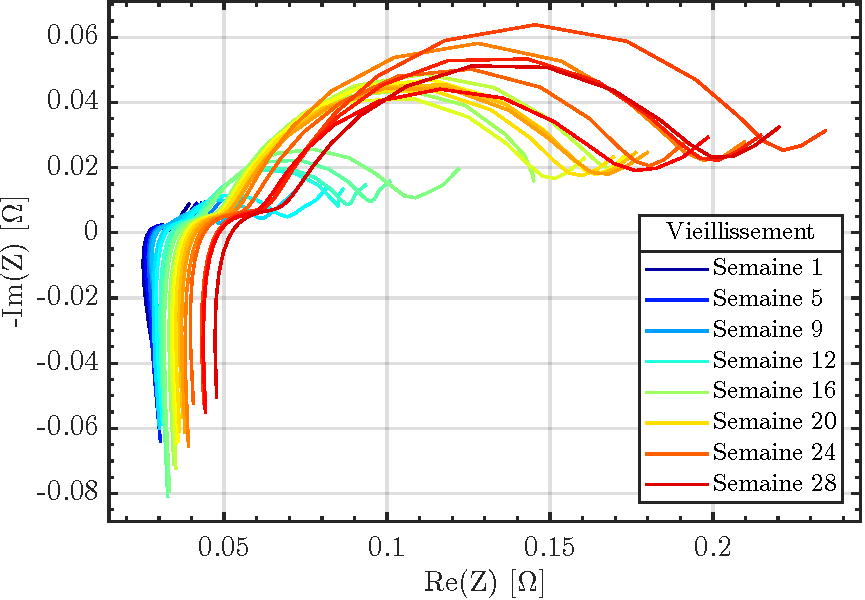
\includegraphics[width=.8\linewidth]{Chapitre 1/Diag_bat/Figures/nyquist_aging_data.pdf}
    \caption{Évolution des diagrammes de Nyquist de la cellule 5 (SoC100) au cours des semaines d'essais}
    \label{nyquist_aging2}
\end{figure}
\FloatBarrier
On observe ainsi bien le décalage des spectres au cours du temps, avec deux caractéristiques principales : le décalage vers la droite des spectres, ainsi que l'élargissement du second dôme. 
Ici, chaque vecteur de données est composé de 32 entrées, qui est un nombre qui permettait d'avoir des résultats interprétables sans que le temps accordé à la mesure (notamment en basse fréquence) ne soit trop important. Ici, un temps de spectroscopie d'une vingtaine de minutes est en accord avec le temps qui pourrait être consacré au diagnostic dans un cas d'application de micro-réseau électrique. \\
Les données des tests HPPC prennent simplement la forme de deux séries temporelles distinctes : une de tension et une de courant, sur toute la durée du test, qui était d'une dizaine de minutes environ (sans compter les périodes de repos initiales et finales) (voir fig. \ref{hppc}). Cette durée de test est également cohérente avec la durée accordable à un diagnostic réel de batterie. Ces données sont échantillonnées à la seconde.

\subsubsection{Traitement des données HPPC \& diagnostic}
\label{traitement_hppc}
Pour les données de ces tests HPPC, la caractéristique principale qui en est extraite est la résistance interne, que l'on peut mesurer comme étant la différence de tension $\Delta U$ divisée par la différence de courant $\Delta I$ au premier instant lorsque la pulsation de courant est appliquée (fig. \ref{current_pulse}). Pour les données de ces tests HPPC, quatre pulsations distinctes ont été appliquées aux cellules de batteries, et donc quatre mesure de résistances internes peuvent être déduites. La résistance interne retenue est alors la moyenne arithmétique des ces quatre mesures. Pour le moment les résultats seront présentés à un état de charge de 100\%. Un exemple des données extraites par cette méthode est présenté en figure \ref{hppc_rint}.
\begin{figure}[h!]
    \begin{minipage}{.51\linewidth}
    \centering
    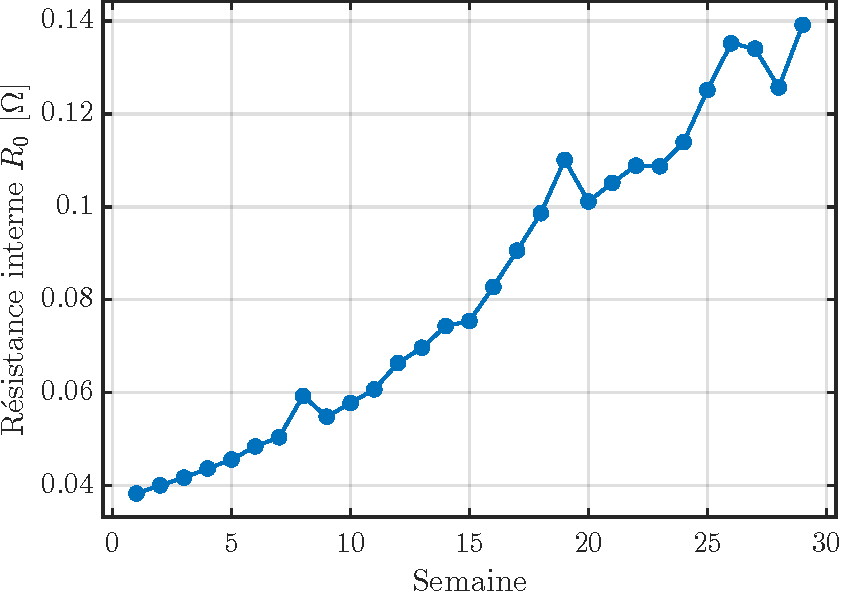
\includegraphics[width=\linewidth]{Chapitre 1/Diag_bat/Figures/hppc_rint.pdf}
    \end{minipage}%
    \hfill
    \begin{minipage}{.48\linewidth}
    \centering
    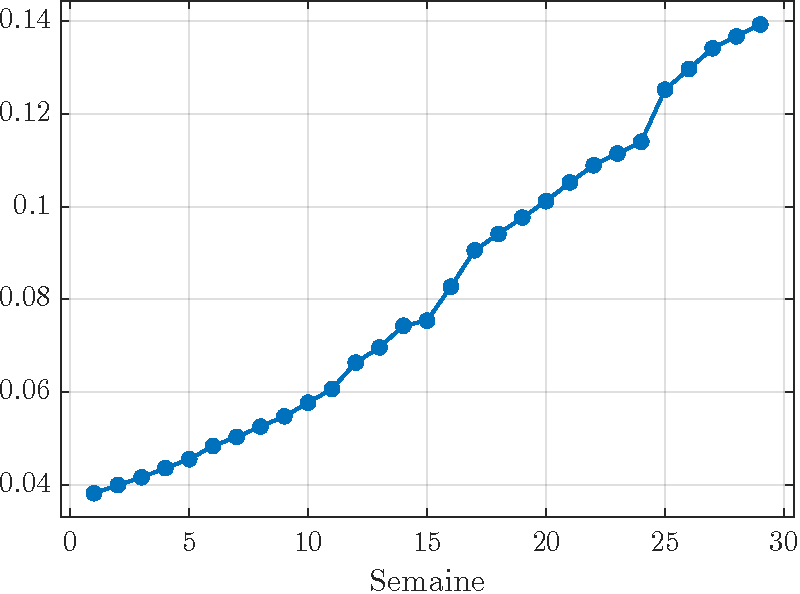
\includegraphics[width=\linewidth]{Chapitre 1/Diag_bat/Figures/hppc_rint_filtered.pdf}
    \end{minipage}
    \caption{Évolution de la résistance interne (HPPC) de la cellule 5 (SoC100) au cours des semaines d'essais (gauche) et filtrée (droite)}
    \label{hppc_rint}
\end{figure}
\FloatBarrier

De la même manière que pour la capacité, ces données peuvent être filtrées à la main pour gommer les mesures aberrantes. Cette étape est également faite par filtrage linéaire (fig. \ref{hppc_rint} droite).

Une fois les données des résistances internes extraites, il est désormais possible de construire des corrélations avec les valeurs de capacité. Un exemple est donné en figure \ref{corr_hppc_rint}.
\begin{figure}[h!]
    \begin{minipage}{.51\linewidth}
    \centering
    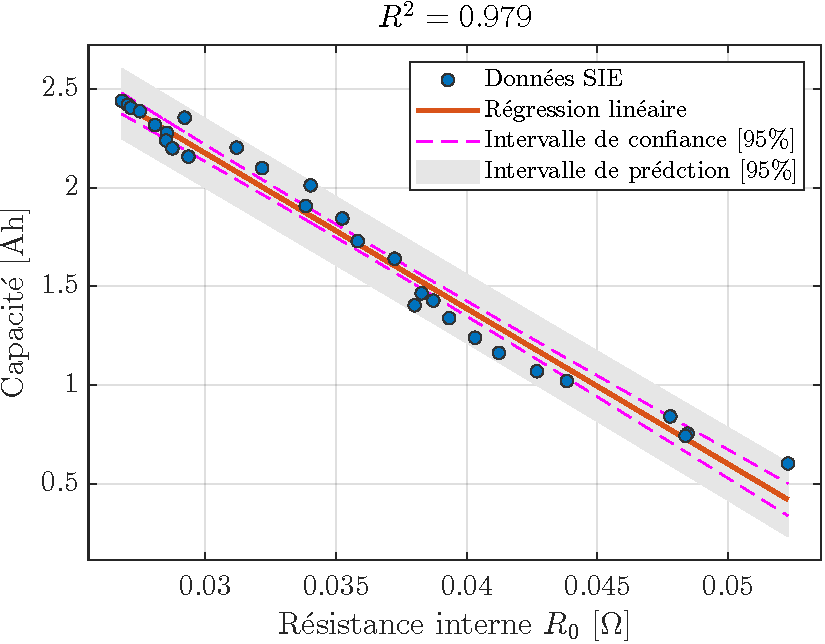
\includegraphics[width=\linewidth]{Chapitre 1/Diag_bat/Figures/corr_hppc_rint.pdf}
    \end{minipage}%
    \hfill
    \begin{minipage}{.48\linewidth}
    \centering
    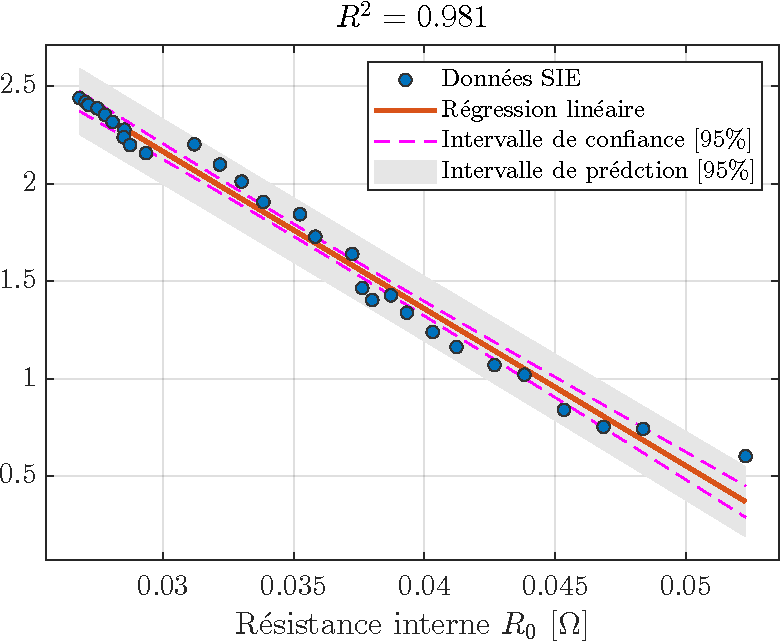
\includegraphics[width=\linewidth]{Chapitre 1/Diag_bat/Figures/corr_hppc_rint_filtered.pdf}
    \end{minipage}
    \caption{Corrélation (HPPC) entre la résistance interne et la capacité de la cellule 5  (gauche) et filtrée (droite)}
    \label{corr_hppc_rint}
\end{figure}
\FloatBarrier
Sur la gauche de cette figure sont représentées les données brutes (pour la cellule 5 à 100\% de SoC), ainsi qu'une régression linéaire par minimisation des carrés des écarts entre les points et la droite de régression. Les intervalles de confiance et de régression à 95\% sont également construits autour de cette droite de régression. L'intervalle de confiance à 95\% indique qu'avec les données présentées ici, il y a 95\% de chances que les paramètres de la droite de régression soient tels que cette droite soit contenue dans l'intervalle de confiance. L'intervalle de confiance est donc un indicateur de la qualité de la régression. L'intervalle de prédiction à 95\% indique que pour une valeur donnée de résistance interne (par exemple), il y a 95\% de chances pour que la valeur de capacité associée soit contenue dans l'intervalle de prédiction. Cet intervalle de prédiction est donc un indicateur de la qualité d'une prédiction de valeur qui serait faire sur la base de cette corrélation. C'est donc celui qui est le plus pertinent pour quantifier l'incertitude dans une approche de diagnostic.

Dans cette figure \ref{corr_hppc_rint}, il est observé que la corrélation entre ces deux grandeurs est alors solide, avec un coefficient de corrélation proche de 1 ainsi qu'un intervalle de confiance resserré autour de la droite de régression. Il est également observé que l'intervalle de prédiction est d'une largeur plutôt constante pour chaque couple de données, sa largeur moyenne valant 0,30Ah. Cela représente une incertitude moyenne de l'ordre 21\% lors d'une prédiction sur la valeur de capacité, avec l'incertitude moyenne qui est définie comme la moyenne des rapports entre les largeurs de l'intervalle de prédiction et les valeurs des capacités pour chaque couple de données. Il apparaît alors que pour ces essais où les capacités ont été poussées très bas (moins de 25\% de la capacité initiale), la largeur de l'intervalle de prédiction constante implique que l'incertitude moyenne est mécaniquement rehaussée. Dans des cas d'applications réelles où ne seraient considérées que les 30\% (par exemple) les plus haut de la capacité de la batterie, l'incertitude moyenne serait par construction plutôt de l'ordre de la dizaine de pourcents, ce qui permet un diagnostic plus fiable.
    
Ces mêmes corrélations peuvent être construites avec les données préalablement filtrées pour ne garder que les données non aberrantes (droite de la figure \ref{corr_hppc_rint}). Il est ici observé que la corrélation est encore plus forte, visible par le coefficient de corrélation qui se rapproche encore de 1 et l'intervalle de confiance se resserrant encore autour de la droite de régression. Cette fois, l'intervalle de prédiction a une largeur moyenne de environ 0,17Ah, ce qui correspond plutôt à une incertitude moyenne sur la capacité de l'ordre de 12\%, en nette baisse par rapport aux données précédentes. Il est notable également qu'en choisissant la même approche que précédemment et en se limitant aux données des 30\% de capacité les plus hauts, l'incertitude moyenne sur la capacité descendrait cette fois en dessous des 10\%. \\ \newline
Cette approche de diagnostic par pulsations de courant semble alors déjà fournir des résultats probants, avec une précision importante et une capacité de prédiction précise. Sa rapidité de mise en oeuvre est également un atout important pour des applications de diagnostic de batteries en situation réelle. Le diagnostic par les méthodes de spectroscopie d'impédance électrochimique est ensuite présenté.

\subsubsection{Traitement des données de SIE \& diagnostic}
\label{sec:diag_sie}
Après la résistance interne simple, il est possible d'estimer d'autres paramètres équivalents pour estimer la capacité de la batterie. En construisant des modèles électriques équivalents de cette batterie, il est ainsi possible d'introduire des paramètres traduisant son comportement. Les approches basées sur la spectroscopie d'impédance permettent notamment de créer et d'ajuster ces paramètres de modèles équivalents \cite{liu_state--health_2023}. Parmi ces paramètres, on peut notamment retrouver la résistance interne ou encore la résistance de transfert de charge \cite{zhang_electrochemical_2022}\cite{nguyen_van_estimation_2023}, présentes dans un circuit équivalent tel que celui de la figure \ref{ecm_bat}.
Une fois le modèle équivalent posé, les valeurs des paramètres choisis peuvent être déterminées. Pour cela, les données récoltées après les tests sont utilisées comme cible à atteindre pour le modèle. L'impédance équivalente du circuit est tout d'abord calculée, fonction de la fréquence : 
\begin{equation}
    Z_{\omega} = j\omega L_s + R_0 + \frac{R_{SEI}}{R_{SEI} + Y_1 (j\omega)^{n_1}} + \frac{R_{ct}}{R_{ct} + Y_2 (j\omega)^{n_2}}
\end{equation}
où ici $\omega = 2\pi f$ est la pulsation, les $Y_i$ représentent les pseudo-capacités des CPE, et les $n_i$ représentent leur exposant de phase. Le vecteur de paramètres suivant peut être tiré :
\begin{equation}
    \beta = \left[ L_s, R_0, R_{SEI}, Y_1, n_1, R_{ct}, Y_2, n_2 \right]
\end{equation}
Pour chaque valeur de fréquence, l'expression théorique fournira une valeur de l'impédance à comparer aux données réelles mesurées. Cette valeur théorique dépend bien sûr de la valeur du vecteur de paramètres $\beta$. 

La méthodes des moindres carrés est maintenant applicable pour ajuster la courbe donnée par cette expression théorique aux données récoltées par la spectroscopie d'impédance. Cet ajustement se fait pour chaque jeu de données correspondant à chaque phase du vieillissement ainsi que chaque niveau d'état de charge. Un exemple de la méthode des moindres carrés appliquées à un diagramme de Nyquist de batterie est donné en figure \ref{least_squares_bat}.
\begin{figure}[h]
\centering
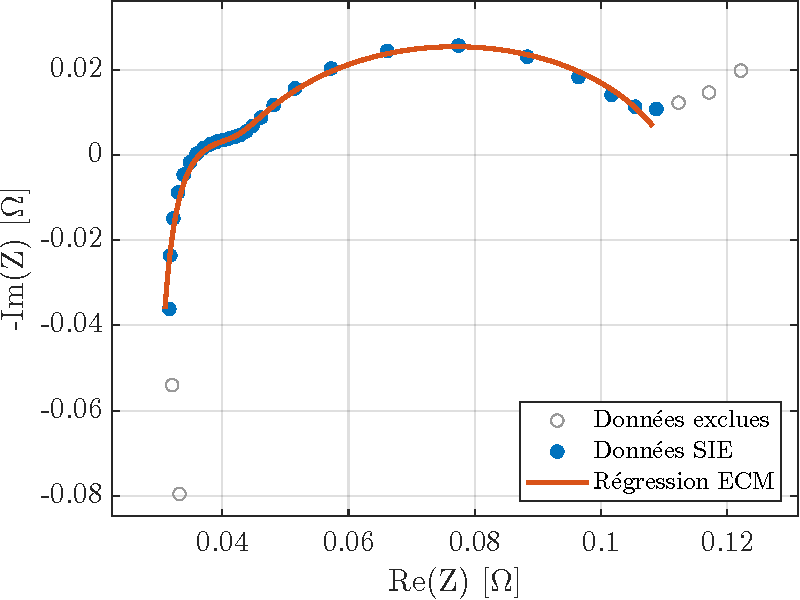
\includegraphics[width=.8\linewidth]{Chapitre 1/Diag_bat/Figures/least_squares_eis.pdf}
\caption{Application de la méthodes des moindres carrés pour l'ajustement du modèle d'impédance aux données de SIE}
\label{least_squares_bat}
\end{figure}
\FloatBarrier
Sur cette figure, des points apparaissent comme ayant servis à la calibration du vecteur de paramètres $\beta$, quand d'autres n'ont pas été utilisés. Cela découle du fait que le modèle utilisé pour construire le spectre d'impédance théorique ne prend pas en compte plusieurs phénomènes physiques, comme le décalage du spectre vers les hautes impédances réelles à haute fréquence, ou encore l'effet de l'impédance de Warburg, qui forme cette droite à environ 45\textdegree \  pour les fréquences les plus basses. Les données ont alors été ajustées pour ne prendre en compte que celles qui sont réellement prédictibles par le modèle. L'algorithme utilisé dans cette méthode des moindres carrés est celui des régions de confiance, qui donne des résultats de convergence généralement meilleurs que les algorithmes de descente de gradient classique. En particulier cet algorithme a donné de meilleurs résultats pour l'ajustement de modèle d'impédance que les algorithmes de Levenberg-Marquardt ou la méthode des points intérieurs. 
Une fois cet ajustement fait, les données correspondant aux paramètres sont accessibles et peuvent alors être mises en comparaison avec les relevés de capacité après chaque période de vieillissement (fig. \ref{capa_cell5}). Les deux paramètres considérés comme potentiellement liés à la capacité de la batterie sont la résistance interne et la résistance de transfert de charge. Le graphe des données de la résistance interne est donné en figure \ref{eis_rint}.
\begin{figure}[h!]
    \begin{minipage}{.51\linewidth}
    \centering
    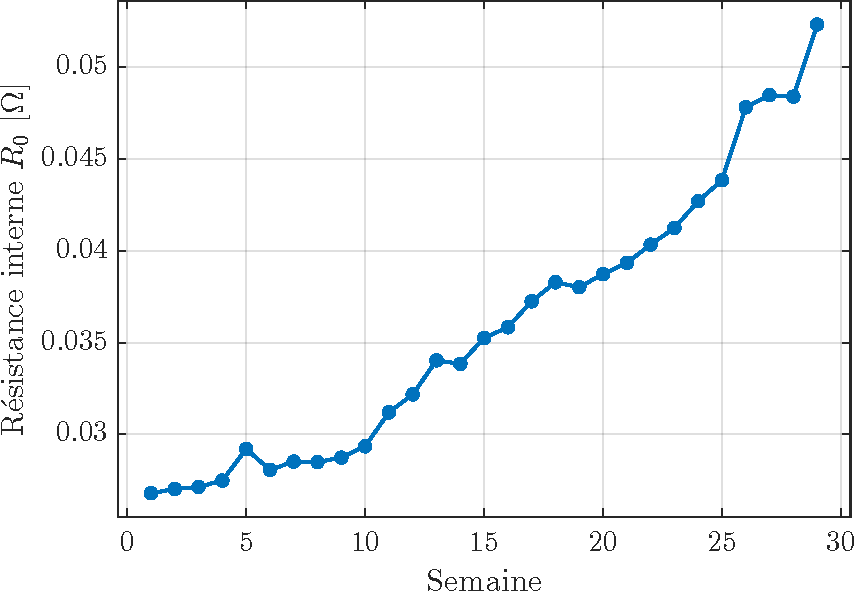
\includegraphics[width=\linewidth]{Chapitre 1/Diag_bat/Figures/eis_rint.pdf}
    \end{minipage}%
    \hfill
    \begin{minipage}{.48\linewidth}
    \centering
    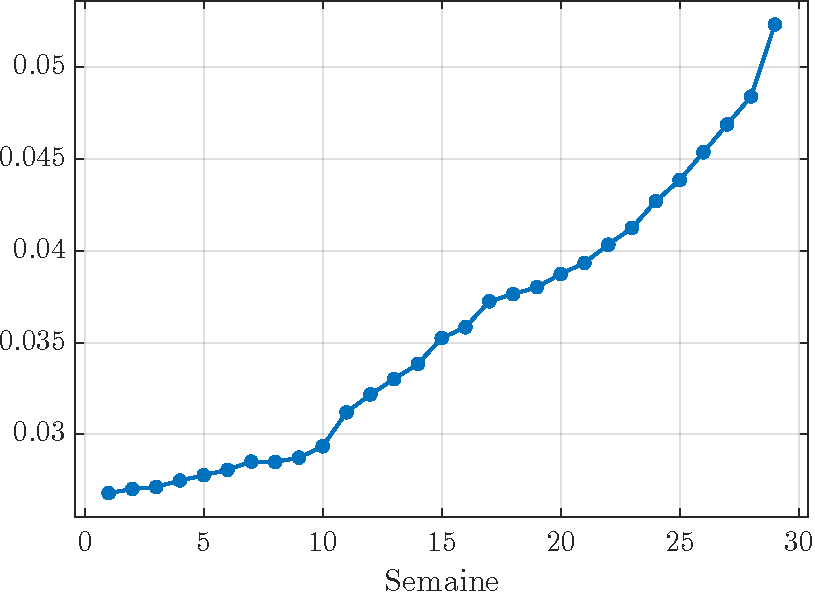
\includegraphics[width=\linewidth]{Chapitre 1/Diag_bat/Figures/eis_rint_filtered.pdf}
    \end{minipage}
    \caption{Évolution de la résistance interne (SIE) de la cellule 5 (SOC100) au cours des semaines d'essais (gauche) et filtrée (droite)}
    \label{eis_rint}
\end{figure}
\FloatBarrier
Il est logique à ce moment de l'étude de remarquer que le graphe de la résistance interne estimée par SIE est similaire au graphe de la résistance interne estimée par HPPC (fig. \ref{hppc_rint}). En effet, c'est le même paramètres avec la même signification physique qui est considéré dans les deux cas, seulement estimé différemment. 

Il est également intéressant désormais d'étudier les données récoltées sur la résistance de transfert de charge, autre paramètre pouvant être relié à la capacité de la batterie \cite{zhang_electrochemical_2022} (fig. \ref{eis_rct}).

\begin{figure}[h!]
    \begin{minipage}{.51\linewidth}
    \centering
    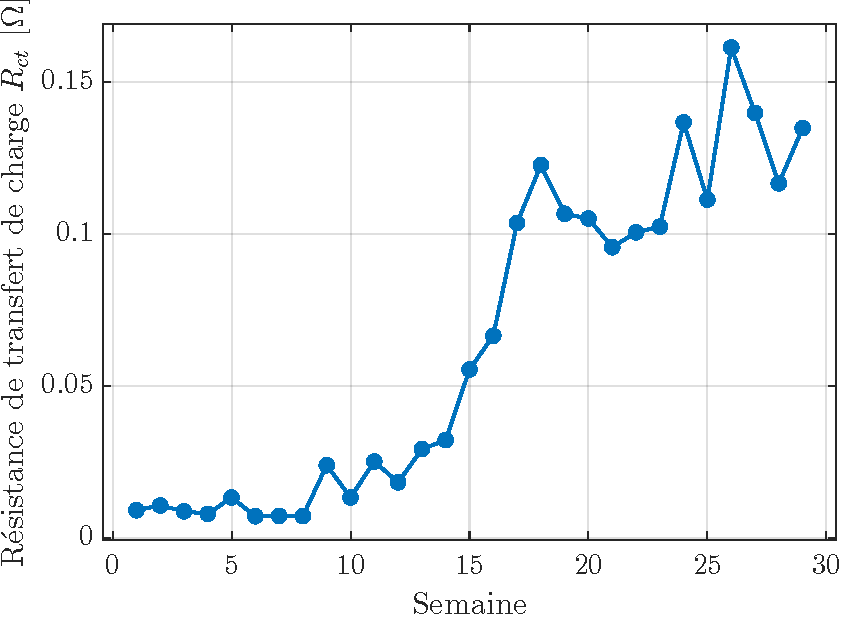
\includegraphics[width=\linewidth]{Chapitre 1/Diag_bat/Figures/eis_rct.pdf}
    \end{minipage}%
    \hfill
    \begin{minipage}{.48\linewidth}
    \centering
    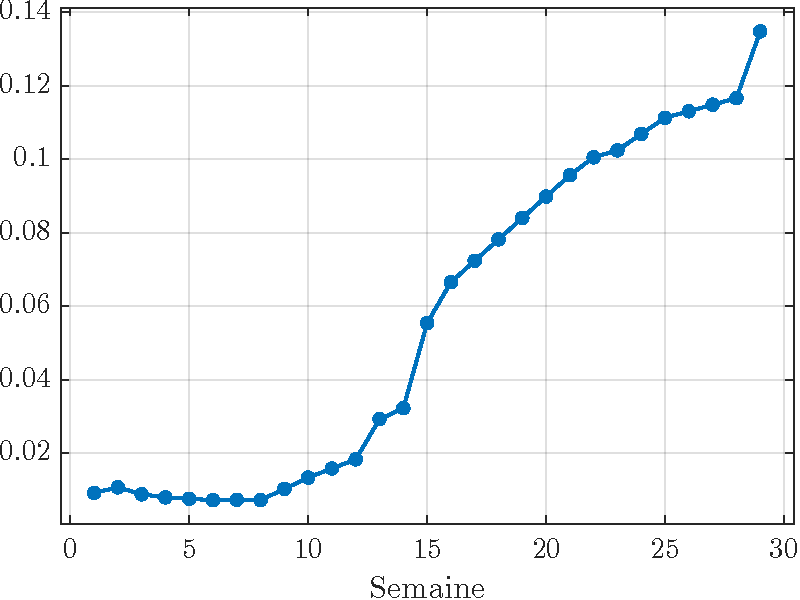
\includegraphics[width=\linewidth]{Chapitre 1/Diag_bat/Figures/eis_rct_filtered.pdf}
    \end{minipage}
    \caption{Évolution de la résistance de transfert de charge (SIE) de la cellule 5 (SOC100) au cours des semaines d'essais (gauche) et filtrée (droite)}
    \label{eis_rct}
\end{figure}
\FloatBarrier
De la même manière qu'avec les données obtenues par la méthode HPPC,  les données sont filtrées sur les quelques points qui semblent être des données aberrantes. Il est à noter cependant que pour la courbe de la résistance de transfert de charge, les profil est beaucoup plus irrégulier ce qui rend le filtrage à la main plus arbitraire, et doit vraisemblablement diminuer la confiance qui doit être accordé à cette méthode. 

Avec les données récoltées sur la capacité ainsi que les données des paramètres équivalents extraites par l'ajustement des paramètres, des corrélations entre ces paramètres sont tracées. Sont tout d'abord étudiées les simples corrélations linéaires entre les différentes grandeurs. En effet, en première approche les deux quantités semblent varier de concert. Un exemple de ces corrélations est donné est figure \ref{corr_eis_rint} avec la résistance interne. 
\begin{figure}[h!]
    \begin{minipage}{.51\linewidth}
    \centering
    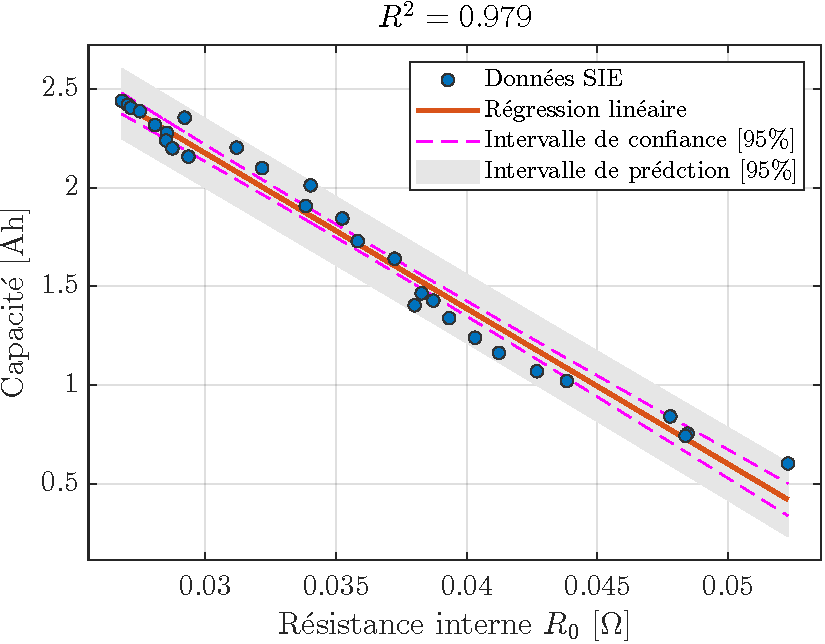
\includegraphics[width=\linewidth]{Chapitre 1/Diag_bat/Figures/corr_eis_rint.pdf}
    \end{minipage}%
    \hfill
    \begin{minipage}{.48\linewidth}
    \centering
    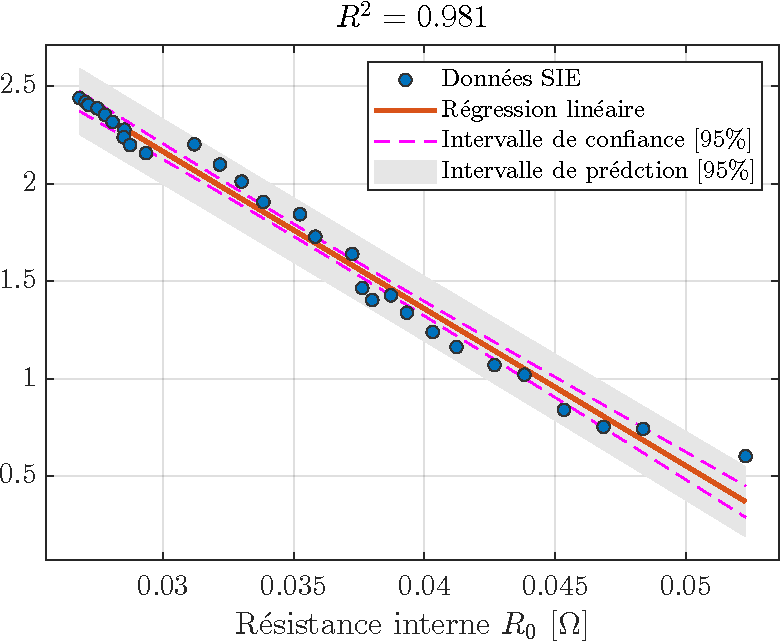
\includegraphics[width=\linewidth]{Chapitre 1/Diag_bat/Figures/corr_eis_rint_filtered.pdf}
    \end{minipage}
    \caption{Corrélation (SIE) entre la résistance interne et la capacité de la cellule 5 (gauche) et filtrée (droite)}
    \label{corr_eis_rint}
\end{figure}
\FloatBarrier

Dans cette régression et comme dans celle apportée par l'approche HPPC, la corrélation entre la capacité et la résistance interne est forte, que ce soit au niveau du coefficient de corrélation ou au niveau de l'intervalle de confiance qui est resserré autour de la droite de régression. Cela confirme que la résistance interne est un bon indicateur pour le diagnostic des batteries. La corrélation entre la capacité et la résistance de transfert de charge est présentée à la figure \ref{corr_eis_rct}.
\begin{figure}[h!]
    \begin{minipage}{.51\linewidth}
    \centering
    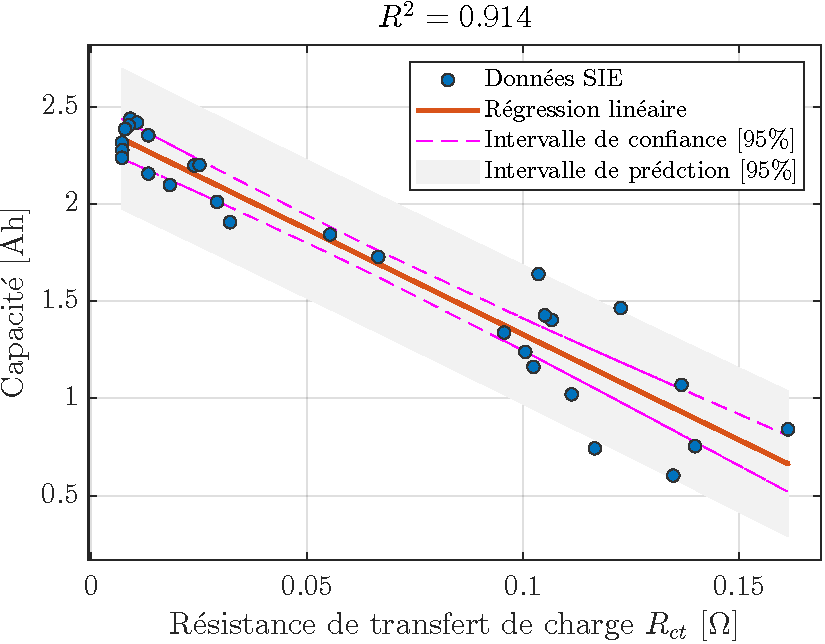
\includegraphics[width=\linewidth]{Chapitre 1/Diag_bat/Figures/corr_eis_rct.pdf}
    \end{minipage}%
    \hfill
    \begin{minipage}{.48\linewidth}
    \centering
    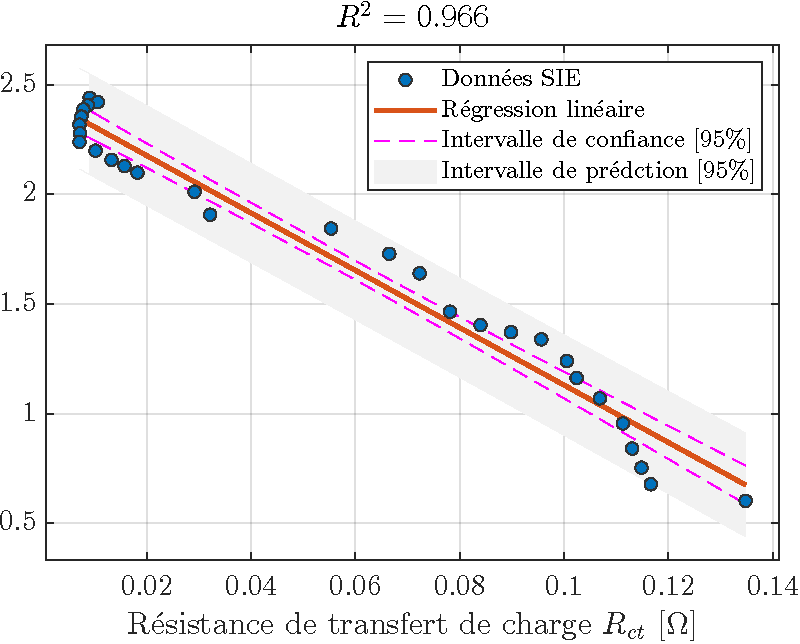
\includegraphics[width=\linewidth]{Chapitre 1/Diag_bat/Figures/corr_eis_rct_filtered.pdf}
    \end{minipage}
    \caption{Corrélation (SIE) entre la résistance de transfert de charge et la capacité de la cellule 5 (gauche) et filtrée (droite)}
    \label{corr_eis_rct}
\end{figure}
\FloatBarrier
La corrélation est ici moins évidente, bien que présente. En effet, le coefficient de corrélation n'est pas du tout aussi proche de 1 que pour la résistance interne, et l'intervalle de confiance est moins resserré autour de la droite de régression. Il est cependant également intéressant de regarder la corrélation entre la résistance de transfert de charge et le logarithme de la capacité, la relation n'étant pas totalement linéaire, notamment dans la littérature \cite{zhang_electrochemical_2022}. Un exemple de cette corrélation est donné en figure \ref{corr_eis_rct_log}.
\begin{figure}[h!]
    \begin{minipage}{.51\linewidth}
    \centering
    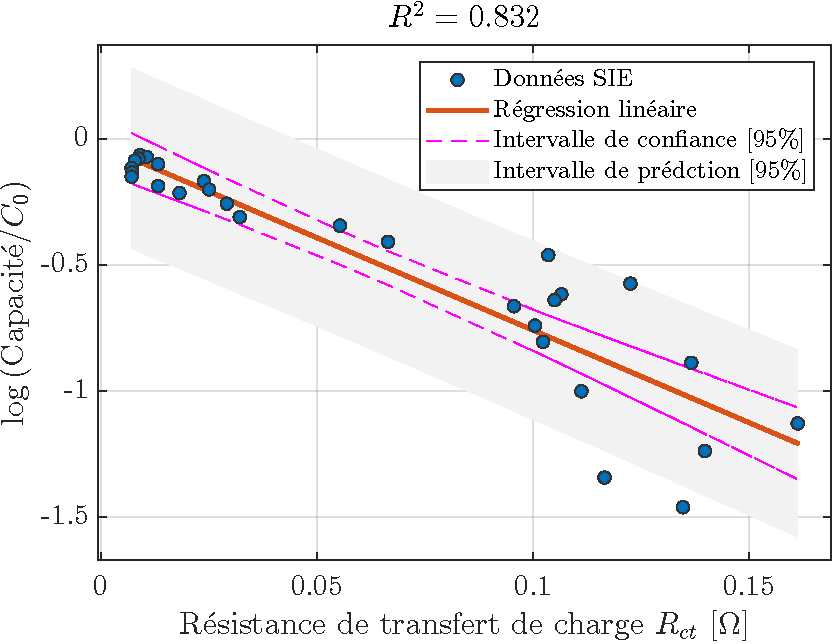
\includegraphics[width=\linewidth]{Chapitre 1/Diag_bat/Figures/corr_eis_rct_log.pdf}
    \end{minipage}%
    \hfill
    \begin{minipage}{.48\linewidth}
    \centering
    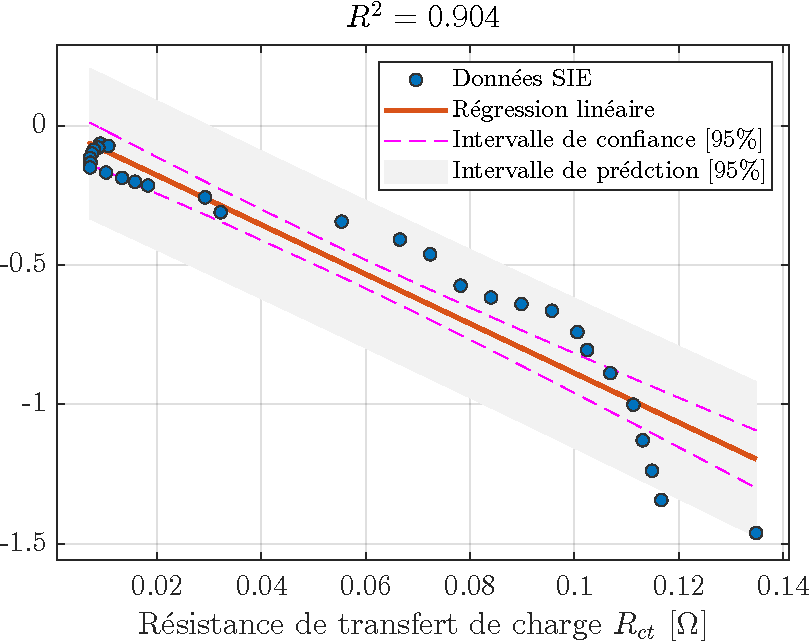
\includegraphics[width=\linewidth]{Chapitre 1/Diag_bat/Figures/corr_eis_rct_log_filtered.pdf}
    \end{minipage}
    \caption{Corrélation (SIE) entre la résistance de transfert de charge et le logarithme de la capacité de la cellule 5 (gauche) et filtrée (droite)}
    \label{corr_eis_rct_log}
\end{figure}
\FloatBarrier
Sur cet exemple, considérer le logarithme de la capacité ne semble pas avoir amélioré la construction de la corrélation. Il semble plutôt que celle-ci s'est détérioré. 
On remarque ainsi que même avec l'ajout d'un filtrage, l'approche considérant la relation logarithmique entre la capacité et la résistance de transfert de charge n'est pas plus intéressante que l'approche classique, même en considérant les données préalablement filtrée. Il est à noter également que l'approche par la résistance de transfert de charge ne semble pas plus pertinente que l'approche par la résistance interne simple. Ce constat est également accentué par le fait que le filtrage des données aberrantes était bien plus arbitraire avec les données des résistances de transfert de charge qu'avec les données de résistance interne, la courbe présentant moins de tendance claire. 

\subsection{Conclusion sur les méthodes de diagnostic de batterie}
Une fois toutes les méthodes de diagnostic présentées (HPPC \& SIE), il est désormais possible de comparer les résultats qu'elles ont fourni et la qualité des corrélations qui en ont découlées. Un récapitulatif de tous les coefficients $R^2$ des corrélations est donné sur le tableau \ref{tab_corr}. 
\begin{table}[h!]
    \caption{Tableau récapitulatif des coefficients de corrélation pour le diagnostic des batteries \vspace{0.02cm}}
    \centering
    \begin{tabular}{|lc||c|c|c|c|}
    \hline
        \multicolumn{2}{|c||}{$R^2$} & CELL4 & CELL5 & CELL6 & MODULE \\ \hline \hline 
        $R_{int}$ &(SIE)& 0.958 & 0.979 & 0.983 & N/A \\ \hline
        $R_{int}$ (filtrée)&(SIE)& 0.964 & 0.981 & 0.984 & N/A \\ \hline
        $R_{ct}$ &(SIE)& 0.962 & 0.914 & 0.929 & N/A\\ \hline
        $R_{ct}$ (filtrée)&(SIE)& 0.970 & 0.966 & 0.965 & N/A\\ \hline
        $R_{ct}$ \& log &(SIE)& 0.962 & 0.832 & 0.845 & N/A \\ \hline
        $R_{ct}$ \& log (filtrée) &(SIE)& 0.981 & 0.904 & 0.915 & N/A \\ \hline
        $R_{int}$ &(HPPC)& 0.983 & 0.984 & 0.980 & 0.969 \\ \hline
        $R_{int}$ (filtrée)&(HPPC)& 0.986 & 0.995 & 0.991 & 0.987 \\ \hline
    \end{tabular}
    \label{tab_corr}
\end{table}
\FloatBarrier
Les données de corrélation obtenus par SIE pour le module de deux cellules ne sont pas renseignées car les données obtenues par cette méthodes ont fourni notamment des résistances internes souvent aberrantes, qui ne permettaient pas de construire de corrélations significatives sans un important filtrage préliminaire. Le reste des données cependant permet de comparer les différentes méthodes de diagnostic, et il apparaît alors que les corrélations obtenues par la méthode HPPC évaluant la résistance interne ont largement fourni les meilleurs résultats, sur toutes les cellules considérées. Il est notable également que cette méthode est la plus rapide à mettre en oeuvre ainsi que la moins coûteuse, puisqu'elle ne nécessite pas l'utilisation d'un spectromètre qui est un appareil qui peut s'avérer onéreux. Cette méthode est donc retenue pour le diagnostic.
De par les données des coefficients de corrélation obtenus, la simple résistance interne est choisie comme indicateur utilisé pour l'estimation de la capacité, et donc de l'état de santé des batteries.

\subsubsection{Discussion}
La méthode de diagnostic des batteries par test HPPC pour la détermination de la résistance interne est la solution choisie. Les graphes des corrélations pour chaque cellules/module sont présentés en figure \ref{corr_hppc_all}.
\begin{figure}[h!]
    \begin{minipage}{.51\linewidth}
    \centering
    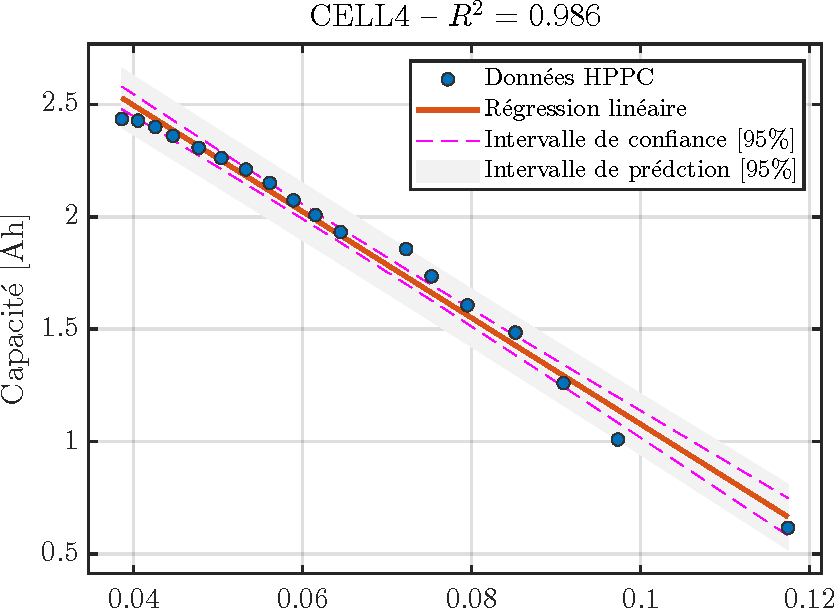
\includegraphics[width=\linewidth]{Chapitre 1/Diag_bat/Figures/corr_hppc_CELL4.pdf}
    \end{minipage}%
    \hfill
    \begin{minipage}{.48\linewidth}
    \centering
    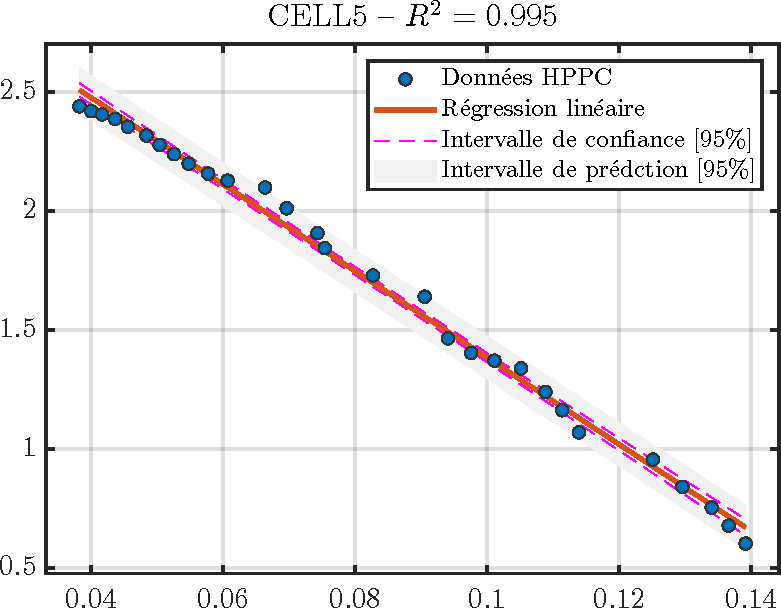
\includegraphics[width=\linewidth]{Chapitre 1/Diag_bat/Figures/corr_hppc_CELL5.pdf}
    \end{minipage}
\end{figure}
\FloatBarrier
\begin{figure}[h!]
    \begin{minipage}{.51\linewidth}
    \centering
    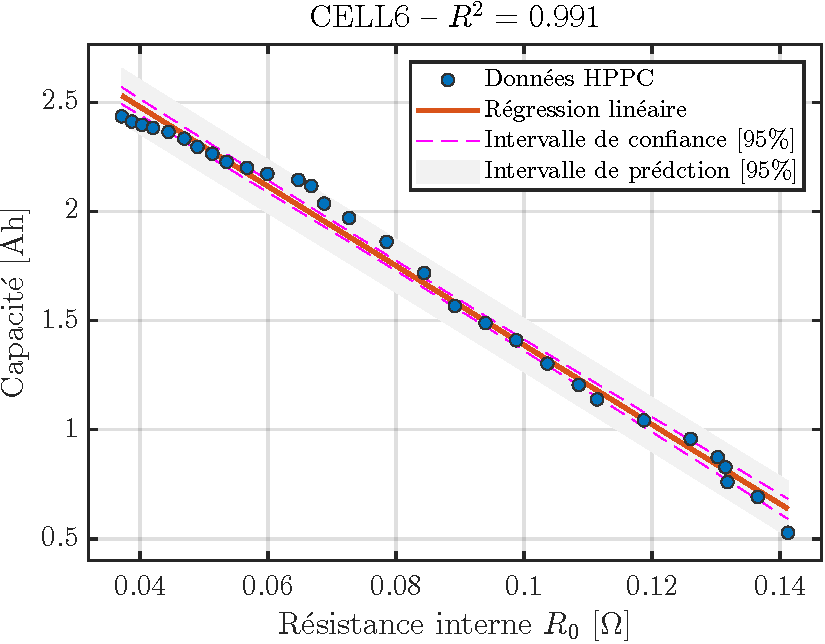
\includegraphics[width=\linewidth]{Chapitre 1/Diag_bat/Figures/corr_hppc_CELL6.pdf}
    \end{minipage}%
    \hfill
    \begin{minipage}{.48\linewidth}
    \centering
    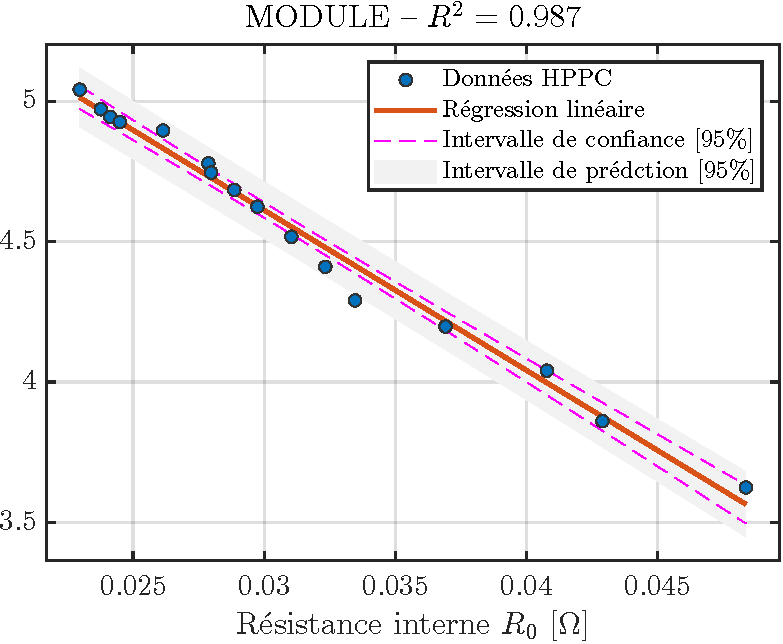
\includegraphics[width=\linewidth]{Chapitre 1/Diag_bat/Figures/corr_hppc_MODULE.pdf}
    \end{minipage}
    \caption{Corrélations entre la capacité et la résistance interne pour tous les systèmes étudiés (HPPC) (filtrées)}
    \label{corr_hppc_all}
\end{figure}
\FloatBarrier
Ces quatre corrélations pour chaque système sont associées à des largeurs d'intervalles de prédictions respectives de 0.26Ah, 0.18Ah, 0.25Ah et 0.21Ah. Ces largeurs d'intervalles correspondent alors à des incertitudes relatives de 10.0\%, 7.0\%, 9.6\% et 4.0\%. Il est ici flagrant que l'incertitude relative pour le module de deux cellules est plus faible. Cela peut s'expliquer par deux observations. Premièrement, il est visible que le module fournit une corrélation basée sur moins de données, celles-ci étant surtout concentrées sur la plage supérieure des capacités (les 30\% supérieurs). Cela est dû aux essais qui ont dû se terminer prématurément sur le module à cause d'une dégradation extérieure qui a altéré ses caractéristiques électriques de manière durable. Ainsi, lorsque l'incertitude relative pour la prédiction est calculée, elle considère des capacités de références relativement élevées, ce qui abaisse mécaniquement la largeur relative de l'intervalle de prédiction. C'est un constat similaire à celui fait dans la partie \ref{traitement_hppc} détaillant la définition de l'intervalle de prédiction. 

Il est remarquable néanmoins que malgré que les capacités soient restreintes à une plage plutôt élevée, la largeur absolue de l'intervalle de prédiction pour le module (0.14Ah) reste dans le même ordre de grandeur que les largeurs des cellules seules (0.20Ah, 0.17Ah et 0.23Ah), alors même que le module est de capacité deux fois plus élevée. Cela soulève donc une question intéressante, qui pourrait être étudiée par la suite : \textbf{est-ce que la largeur de l'intervalle de prédiction est indépendante de la taille du système ?} Et donc, en question sous-jacente : \textbf{est-ce qu'une approche à l’échelle du module ou du pack permettrait d'affiner le diagnostic ?} Ce travail n'a pas vocation à répondre à ces questions qui sont donc laissée en suspens pour le moment. 

Une dernière remarque se pose sur la construction du test HPPC telle que présentée ici. Le choix a été fait d'une multitude de pulsations de courant, d'amplitudes et de signes variés. Avoir cette diversité permet d'affiner le diagnostic et ainsi d'avoir plusieurs mesures de résistances internes à cumuler. Elle est cependant logiquement plus chronophage. Une autre question que soulève ce travail est alors : \textbf{est-ce que l'estimation de la résistance interne peut être rendue encore moins intrusive en réduisant le nombre de pulsations de courant ?} De la même manière, cette question reste en suspens dans le cadre de ce travail.

\subsubsection{Limitations}
Bien que l'utilisation des pulsations de courant ainsi que la spectroscopie d'impédance électrochimique fournissent des résultats intéressants dans le cadre du diagnostic des batteries, cette approche présente tout de même des limitations. En effet, il y a deux problèmes majeurs à cette approche et notamment sur la construction des essais pour la récolte des données sur le comportement des batteries. Ces essais ont eu lieu sans contrôle de la température, tout comme les modèles électriques considérés ne prennent en compte que les phénomènes électriques. C'est une limitation claire alors que l'impact de la température sur le comportement électro-chimique des batteries est établi. La solution logique pour pallier ce problème serait de multiplier les essais en les effectuant avec une température contrôlée, afin d'augmenter la dépendance des modèles en la température et en pouvant ainsi affiner le diagnostic pour le faire dépendre de la température lors de l'essai. 

Une autre limitation importante due à la construction des essais est la partie sur les essais de vieillissement accélérés (AST). En effet, ceux-ci ont été construits avec un cyclage à courant constant pour dégrader les batteries, ce qui ne correspond qu'à peu de cas réels et en particulier ne correspond pas à des profils de puissance d'habitations dans un micro-réseau où les batteries servent de stockage à court-terme. Cela gomme les effets de courants dynamiques et en particulier des pics de courant à haute intensité qui sont connus pour avoir des effets très dégradants sur les batteries. Une solution potentielle à cette limitation est donc de réaliser de nouveaux essais de vieillissement où la dégradation des batteries n'est peut être pas imposée par des cyclages à courant constant, mais plutôt des profils à courant dynamiques, éventuellement reproduisant les profils réels.

\newpage